%%%%%%%%%%%%%%%%%%%%%%%%%%%%%%%%%%%%%%%%%
% Masters/Doctoral Thesis 
% LaTeX Template
% Version 2.5 (27/8/17)
%
% This template was downloaded from:
% http://www.LaTeXTemplates.com
%
% Version 2.x major modifications by:
% Vel (vel@latextemplates.com)
%
% This template is based on a template by:
% Steve Gunn (http://users.ecs.soton.ac.uk/srg/softwaretools/document/templates/)
% Sunil Patel (http://www.sunilpatel.co.uk/thesis-template/)
%
% Template license:
% CC BY-NC-SA 3.0 (http://creativecommons.org/licenses/by-nc-sa/3.0/)
%
%%%%%%%%%%%%%%%%%%%%%%%%%%%%%%%%%%%%%%%%%

%----------------------------------------------------------------------------------------
%	PACKAGES AND OTHER DOCUMENT CONFIGURATIONS
%----------------------------------------------------------------------------------------

\documentclass[
11pt, % The default document font size, options: 10pt, 11pt, 12pt
%oneside, % Two side (alternating margins) for binding by default, uncomment to switch to one side
english, % ngerman for German
singlespacing, % Single line spacing, alternatives: onehalfspacing or doublespacing
%draft, % Uncomment to enable draft mode (no pictures, no links, overfull hboxes indicated)
%nolistspacing, % If the document is onehalfspacing or doublespacing, uncomment this to set spacing in lists to single
%liststotoc, % Uncomment to add the list of figures/tables/etc to the table of contents
%toctotoc, % Uncomment to add the main table of contents to the table of contents
%parskip, % Uncomment to add space between paragraphs
%nohyperref, % Uncomment to not load the hyperref package
headsepline, % Uncomment to get a line under the header
%chapterinoneline, % Uncomment to place the chapter title next to the number on one line
%consistentlayout, % Uncomment to change the layout of the declaration, abstract and acknowledgements pages to match the default layout
]{MastersDoctoralThesis} % The class file specifying the document structure

\usepackage{listings}

\usepackage[utf8]{inputenc} % Required for inputting international characters
\usepackage[T1]{fontenc} % Output font encoding for international characters

\usepackage{amsmath}

\usepackage{mathpazo} % Use the Palatino font by default

\usepackage[backend=bibtex,style=authoryear,natbib=true]{biblatex} % Use the bibtex backend with the authoryear citation style (which resembles APA)

\addbibresource{references.bib} % The filename of the bibliography

\usepackage[autostyle=true]{csquotes} % Required to generate language-dependent quotes in the bibliography

%----------------------------------------------------------------------------------------
%	MARGIN SETTINGS
%----------------------------------------------------------------------------------------

\geometry{
	paper=a4paper, % Change to letterpaper for US letter
	inner=2.5cm, % Inner margin
	outer=3.8cm, % Outer margin
	bindingoffset=.5cm, % Binding offset
	top=1.5cm, % Top margin
	bottom=1.5cm, % Bottom margin
	%showframe, % Uncomment to show how the type block is set on the page
}

%----------------------------------------------------------------------------------------
%	THESIS INFORMATION
%----------------------------------------------------------------------------------------

\thesistitle{Thesis Title} % Your thesis title, this is used in the title and abstract, print it elsewhere with \ttitle
\supervisor{Dr. Robert \textsc{Henderson}} % Your supervisor's name, this is used in the title page, print it elsewhere with \supname
\examiner{} % Your examiner's name, this is not currently used anywhere in the template, print it elsewhere with \examname
\degree{Masters of Science} % Your degree name, this is used in the title page and abstract, print it elsewhere with \degreename
\author{Ragheb \textsc{Al-Ghezi}} % Your name, this is used in the title page and abstract, print it elsewhere with \authorname
\addresses{} % Your address, this is not currently used anywhere in the template, print it elsewhere with \addressname

\subject{Biological Sciences} % Your subject area, this is not currently used anywhere in the template, print it elsewhere with \subjectname
\keywords{} % Keywords for your thesis, this is not currently used anywhere in the template, print it elsewhere with \keywordnames
\university{\href{http://www.university.com}{University Name}} % Your university's name and URL, this is used in the title page and abstract, print it elsewhere with \univname
\department{\href{http://department.university.com}{Department or School Name}} % Your department's name and URL, this is used in the title page and abstract, print it elsewhere with \deptname
\group{\href{http://researchgroup.university.com}{Research Group Name}} % Your research group's name and URL, this is used in the title page, print it elsewhere with \groupname
\faculty{\href{http://faculty.university.com}{Faculty Name}} % Your faculty's name and URL, this is used in the title page and abstract, print it elsewhere with \facname

\AtBeginDocument{
\hypersetup{pdftitle=\ttitle} % Set the PDF's title to your title
\hypersetup{pdfauthor=\authorname} % Set the PDF's author to your name
\hypersetup{pdfkeywords=\keywordnames} % Set the PDF's keywords to your keywords
}

\begin{document}

\frontmatter % Use roman page numbering style (i, ii, iii, iv...) for the pre-content pages

\pagestyle{plain} % Default to the plain heading style until the thesis style is called for the body content

%----------------------------------------------------------------------------------------
%	TITLE PAGE
%----------------------------------------------------------------------------------------

\begin{titlepage}
\begin{center}

\vspace*{.06\textheight}
{\scshape\LARGE \univname\par}\vspace{1.5cm} % University name
\textsc{\Large Doctoral Thesis}\\[0.5cm] % Thesis type

\HRule \\[0.4cm] % Horizontal line
{\huge \bfseries \ttitle\par}\vspace{0.4cm} % Thesis title
\HRule \\[1.5cm] % Horizontal line
 
\begin{minipage}[t]{0.4\textwidth}
\begin{flushleft} \large
\emph{Author:}\\
\href{http://www.johnsmith.com}{\authorname} % Author name - remove the \href bracket to remove the link
\end{flushleft}
\end{minipage}
\begin{minipage}[t]{0.4\textwidth}
\begin{flushright} \large
\emph{Supervisor:} \\
\href{http://www.jamessmith.com}{\supname} % Supervisor name - remove the \href bracket to remove the link  
\end{flushright}
\end{minipage}\\[3cm]
 
\vfill

\large \textit{A thesis submitted in fulfillment of the requirements\\ for the degree of \degreename}\\[0.3cm] % University requirement text
\textit{in the}\\[0.4cm]
\groupname\\\deptname\\[2cm] % Research group name and department name
 
\vfill

{\large \today}\\[4cm] % Date
%\includegraphics{Logo} % University/department logo - uncomment to place it
 
\vfill
\end{center}
\end{titlepage}

%----------------------------------------------------------------------------------------
%	DECLARATION PAGE
%----------------------------------------------------------------------------------------

%\begin{declaration}
%\addchaptertocentry{\authorshipname} % Add the declaration to the table of contents
%\noindent I, \authorname, declare that this thesis titled, \enquote{\ttitle} and the work presented in it are my own. I confirm that:
%
%\begin{itemize} 
%\item This work was done wholly or mainly while in candidature for a research degree at this University.
%\item Where any part of this thesis has previously been submitted for a degree or any other qualification at this University or any other institution, this has been clearly stated.
%\item Where I have consulted the published work of others, this is always clearly attributed.
%\item Where I have quoted from the work of others, the source is always given. With the exception of such quotations, this thesis is entirely my own work.
%\item I have acknowledged all main sources of help.
%\item Where the thesis is based on work done by myself jointly with others, I have made clear exactly what was done by others and what I have contributed myself.\\
%\end{itemize}
% 
%\noindent Signed:\\
%\rule[0.5em]{25em}{0.5pt} % This prints a line for the signature
% 
%\noindent Date:\\
%\rule[0.5em]{25em}{0.5pt} % This prints a line to write the date
%\end{declaration}

\cleardoublepage

%----------------------------------------------------------------------------------------
%	QUOTATION PAGE
%----------------------------------------------------------------------------------------

\vspace*{0.2\textheight}

\noindent\enquote{\itshape Thanks to my solid academic training, today I can write hundreds of words on virtually any topic without possessing a shred of information, which is how I got a good job in journalism.}\bigbreak

\hfill Dave Barry

%----------------------------------------------------------------------------------------
%	ABSTRACT PAGE
%----------------------------------------------------------------------------------------

\begin{abstract}
\addchaptertocentry{\abstractname} % Add the abstract to the table of contents
The Thesis Abstract is written here (and usually kept to just this page). The page is kept centered vertically so can expand into the blank space above the title too\ldots
\end{abstract}

%----------------------------------------------------------------------------------------
%	ACKNOWLEDGEMENTS
%----------------------------------------------------------------------------------------

\begin{acknowledgements}
\addchaptertocentry{\acknowledgementname} % Add the acknowledgements to the table of contents
The acknowledgments and the people to thank go here, don't forget to include your project advisor\ldots
\end{acknowledgements}

%----------------------------------------------------------------------------------------
%	LIST OF CONTENTS/FIGURES/TABLES PAGES
%----------------------------------------------------------------------------------------

\tableofcontents % Prints the main table of contents

\listoffigures % Prints the list of figures

\listoftables % Prints the list of tables

%----------------------------------------------------------------------------------------
%	ABBREVIATIONS
%----------------------------------------------------------------------------------------

\begin{abbreviations}{ll} % Include a list of abbreviations (a table of two columns)

\textbf{LAH} & \textbf{L}ist \textbf{A}bbreviations \textbf{H}ere\\
\textbf{WSF} & \textbf{W}hat (it) \textbf{S}tands \textbf{F}or\\

\end{abbreviations}

%----------------------------------------------------------------------------------------
%	PHYSICAL CONSTANTS/OTHER DEFINITIONS
%----------------------------------------------------------------------------------------

%\begin{constants}{lr@{${}={}$}l} % The list of physical constants is a three column table
%
%% The \SI{}{} command is provided by the siunitx package, see its documentation for instructions on how to use it
%
%Speed of Light & $c_{0}$ & \SI{2.99792458e8}{\meter\per\second} (exact)\\
%%Constant Name & $Symbol$ & $Constant Value$ with units\\
%
%\end{constants}

%----------------------------------------------------------------------------------------
%	SYMBOLS
%----------------------------------------------------------------------------------------

%\begin{symbols}{lll} % Include a list of Symbols (a three column table)
%
%$a$ & distance & \si{\meter} \\
%$P$ & power & \si{\watt} (\si{\joule\per\second}) \\
%%Symbol & Name & Unit \\
%
%\addlinespace % Gap to separate the Roman symbols from the Greek
%
%$\omega$ & angular frequency & \si{\radian} \\
%
%\end{symbols}

%----------------------------------------------------------------------------------------
%	DEDICATION
%----------------------------------------------------------------------------------------

\dedicatory{For/Dedicated to/To my\ldots} 

%----------------------------------------------------------------------------------------
%	THESIS CONTENT - CHAPTERS
%----------------------------------------------------------------------------------------

\mainmatter % Begin numeric (1,2,3...) page numbering

\pagestyle{thesis} % Return the page headers back to the "thesis" style

% Include the chapters of the thesis as separate files from the Chapters folder
% Uncomment the lines as you write the chapters

% Chapter Template

\chapter{Text Representation} % Main chapter title

\label{Chapter1} % Change X to a consecutive number; for referencing this chapter elsewhere, use \ref{ChapterX}

%----------------------------------------------------------------------------------------
%	SECTION 1
%----------------------------------------------------------------------------------------

\section{Introduction} 

Computers do not understand human language the way we do; they are limited by their innate nature of numerical computation. So in order to make use of decades worth of lingusitic theories in the field of human language technology, tremendious human efforts must be extended to represent lingusitic phenomona in a way computers are able to deal with. The goal is to unify the representation of textual documents
whatever their formats by transforming them into a set of terms
(features) that can be easily used by learning algorithms. Features can be thought of as any rule a lingusit devises to represent particular characteristic of langauge. For instance, the presence of the substring `win \$1000 by clicking here` in an email may indicate for its spamminess. Feature engineering and design is an active research area in natural language processing, and its methods spans between manual and automatic creation.

In order to apply learning algorithms on text, it is necessary to create
a numerical representation of the text and assign a weight to each
feature in text. This weighting is extremely important as it will
influence the results of learning algorithms. Thus, a second objective
is to improve weight the features.

The number of features is a very important factor on which the
performance of Text Classification depends. Indeed, several learning
algorithms are unable to handle a large number of features. For this
purpose, it is necessary to reduce the dimensionality of the
representation space by keeping only the best features. Reduction
methods are used to select or extract the most important features. In
this chapter, we present most common automatic methods of text
representation, specifying their advantages and disadvantages, and then we
discuss the weighting techniques most used in Text Classification as
well as the techniques used to reduce dimensionality.

\section{Classification as a Machine Learning Task}
Classification is a supervised Machine learning task aims to select a correct class for a given input, or more generally a task of “ assigning objects from a universe to two or more classes or categories ” \citep{manning1999foundations}. In natural language processing, the tasks of tagging, word sense disambiguation and spam filtering are all examples of supervised machine learning classification. A classifier is an algorithm that quantitatively models the relationship between a set of inputs and their associated output such that it generalizes well to new input data. In the task of spam filtering, for instance, input data are set of sentences with binary labels (SPAM, Not SPAM). 

\textbf{CHECKMEOUT}: There are two main phases to supervised classification: Training and Prediction. During training, a feature extractor is used to convert each input value to a feature set. These feature sets, which capture the basic information about each input that should be used to classify it, are discussed in the next section. Pairs of feature sets and labels are fed into the machine learning algorithm to generate a model. In prediction phase, the same feature extractor is used to convert unseen inputs to feature sets. These feature sets are then fed into the model, which generates predicted labels.

\begin{figure}
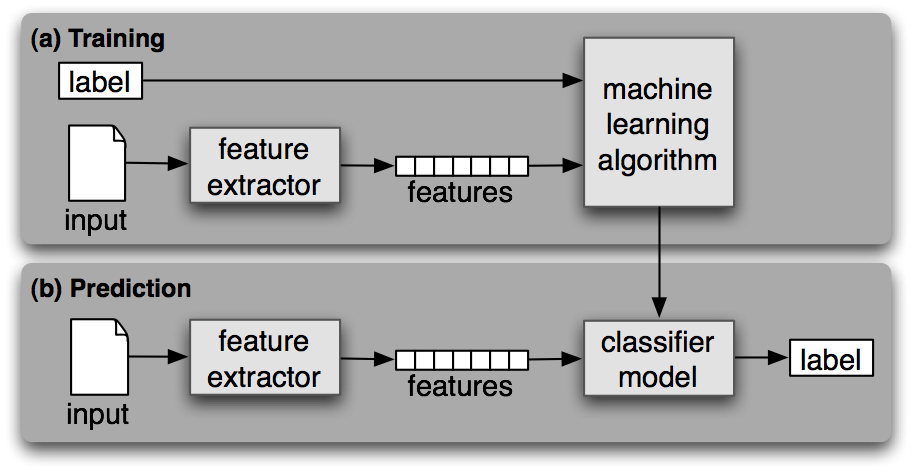
\includegraphics[scale=.8]{../Figures/mlpipeline.png} \centering
\caption{A figure shows the machine learning workflow}
\end{figure}

 \section{Logistic Regression}
 Logistic regression is one of the most common machine learning classifier in natural language processing tasks. It is also considered the building blocks of neural network models. Logistic regression belongs to a group of probabilistic classifiers called discriminative models which, unlike its generative counterparts like Naive Bayes classifiers, is to try to learn to distinguish the classes. More formally, given a document $d$ and a class $c$ , logistic regressions attempts to compute the conditional probability $P(c|d)$. 
 According to \citep{jurafsky2014speech}, classification using logistic regression, like any other supervised classification algorithm, has four main components: 

\begin{list}{•}{}
 \item Feature Representation: a method of numerically represent language data (characters, words and sentences, etc) input $x$ as feature vector $[x_{1},x_{2},x_{3},...x_{n}]$ where $i$  represents an observation in the input data.

\item Classification function: computes an estimation to class $\hat{y}$ via $p(y|x)$. In the case of binary logistic regression, the sigmoid function is used, while a softmax is used for multinomial classification. 
 
\item An objective function involving minimizing error on training examples (cross entropy)

\item An optimizer to help find the minimum of objective function 
 (stochastic gradient descent).
 \end{list}

Logistic regression also has two phases: training and testing. In training phase, the goal is to find the optimal weights that best account for mapping input features $x_{i}$ to the labelled output $y_{i}$ of a subset of the data. In testing, we measure the generalizability of weights learned in the training phase on the remaining set of the data.

Given a dataset $\mathcal { D } = \left\{ \left( \boldsymbol { x } ^ { ( i ) } , y ^ { ( i ) } \right) \right\} _ { i = 1 } ^ { N }$, the weights  are estimated by maximum conditional likelihood, 

\begin{equation}
\log \mathrm { p } \left( \boldsymbol { y } ^ { ( 1 : N ) } | \boldsymbol { x } ^ { ( 1 : N ) } ; \boldsymbol { \theta } \right) = \sum _ { i = 1 } ^ { N } \log \mathrm { p } \left( y ^ { ( i ) } | \boldsymbol { x } ^ { ( i ) } ; \boldsymbol { \theta } \right)
\end{equation}
\begin{equation}
\sum _ { i = 1 } ^ { N } \boldsymbol { \theta } \cdot \boldsymbol { f } \left( \boldsymbol { x } ^ { ( i ) } , y ^ { ( i ) } \right) - \log \sum _ { y ^ { \prime } \in \mathcal { Y } } \exp \left( \boldsymbol { \theta } \cdot \boldsymbol { f } \left( \boldsymbol { x } ^ { ( i ) } , y ^ { \prime } \right) \right)
\end{equation}





\section{Feature Representation}

A feature is defined as any element that can be used as an attribute in classification algorithms. Choosing what features to use to represent a text or a document not only has a major impact on the entire classification process, but it is also arguably the most difficult phase in any natural language processing task. The reasons go to several fundamental questions on how to represent language computationally. For example, on what level should we represent a text: \emph{character-wise}, \emph{word-wise} or \emph{sentence-wise}, or even more specifically morphologically, etymologically or phonologically? Do we treat a word e.g. \emph{try} and all its morphological variations e.g. \emph{tries}, \emph{trying}, \emph{tried} similarly or differently? How to represent and model the semantics of human language computationally? Questions like these and many others are the core of natural language processing; therefore, we briefly explore some of the most common text representation methods.

\subsection{Frequency-based Methods}

\subsubsection{Bag-of-Words Representation}

The "bag of words" representation is the simplest and most intuitive
representation. It represents each document by a vector
whose component corresponds to the number of occurrences of a word in
the document.  Words have the advantage of having an
explicit meaning. Nevertheless, the implementation of this
representation raises several difficulties. The first difficulty is that
of the delimitation of words in a text. Indeed, we still can not define
what is a word. A word as being a sequence of
characters belonging to a dictionary, or formally, as being a sequence
of characters separated by spaces or punctuation characters. This
definition is not valid for all languages. Indeed, languages such as
Chinese or Japanese do not separate their words by spaces. In addition, some separators can be part of certain words (for example: today,
127.0.0.1, potato, etc.). Another difficulty concerns the management of
compound words (for example: rainbow, potato, etc.) and acronyms (like:
IBM, CAF, CAN, etc.). Consideration of these cases requires quite
complex language treatments. This representation of texts excludes any
grammatical analysis and any notion of order between words and therefore
semantically distant texts can have the same representation. For
example, the sentences \texttt{the\ wolf\ eats\ the\ goat} and
\texttt{the\ goat\ eats\ the\ wolf} is given the same representation
despite being semantically different.

% \subsubsection{Representation by Sentences}

Bag-of-words representation excludes any notion of order and
relationship between the words of a text, several studies have
attempted to use sentences as features instead of words \citep{fuhr1991probabilistic} \citep{tzeras1993automatic}.
The use of the sentences makes it possible to solve the problem of
ambiguity generated by the use of the representation "bag of words". For
example, the word \texttt{mouse} has several possible meanings while
optical mouse and domestic mouse has no ambiguity. Although the
sentences have the advantage of better keeping the semantics in relation
to the words, their use as features did not lead to the expected
results. According to Lewis \citep{lewis1992representation}, this representation is penalized
by the large number of possible combinations which leads to low and too
random frequencies. One solution proposed in \citep{caropreso2001learner} was to consider a
sentence as a set of contiguous (but not necessarily ordered) words that
appear together but do not necessarily respect grammatical rules.

% \subsubsection{Representation by lemmas or lexical roots}

A modification to the "bag of words" is representation by lemmas or lexical roots which replaces  each word by its canonical form so that words with different
forms (singular, plural, masculine, feminine, present, past,
future, etc.) can have in a single form called a canonical form.
Grouping the different forms of a word offers the advantage of  reducing the dimensionality of the learning space. Indeed, in the bag-of-words representation, each form of a word is given a dimension; while with lemma representation the different forms of one word will be merged into one dimension. For example, words such as play, player, players, play, play, play, cheek, etc. will be replaced by a single describer ie the root played or the lemma play.


Lemmatization and stemming are the two techniques used to find the canonical form of a word. Lemmatization uses a knowledge base containing the different inflected forms corresponding to the different possible lemmas. Thus, the inflected forms of a noun will be replaced by the singular masculine form while the different inflected forms of a verb will be replaced by the infinitive form. Lemmatization requires the use of a dictionary of inflected forms of language as well as a grammar labeler. An efficient algorithm, named TreeTagger \citep{schmid1994probabilistic}, has been developed for thirteen different languages: German, English, French, Italian, Dutch, Spanish, Bulgarian, Russian, Greek, French Portuguese, Chinese, Swahili and Old French. Stemming uses a knowledge base of syntactic and morphological rules and to transform words into their roots. One of the most well-known stemming algorithms for the English language is Porter's algorithm \citep{porter1980algorithm}. Lemmatization is more complicated to implement since it depends on the grammatical labellers. In addition, it is more sensitive to misspellings than stemming.

\begin{lstlisting}[language=Python, caption=Python example]
def stem(word):
    Suffix_list = ["ing","ly","ed","ious",\
				"ies","ive","es","s","ment"]
    for suffix in Suffix_list:
        if word.endswith(suffix):
            return word[:-len(suffix)]
    return word
\end{lstlisting}

% \subsubsection{Representation by n-grams}

A slightly better approach to represent text that makes use of context is the representation by n-grams. It consists of breaking the text into moving sequences of $n$ consecutive tokens. For example, the trigram segmentation of the word "language" gives the following 3-grams: lan, ang, ngu, gua, uag, age. The notion of n-grams was introduced by  \citep{shannon1948mathematical}; he was interested in predicting the appearance of certain characters according to the other characters. Since then, n-grams have been used in many areas such as speech recognition, documentary research, and so on. The use of n-grams offers the following advantages: 1) language-independent 2) Requiring no prior segmentation of the document. 3) Less sensitive to misspellings. 4) effective method to automatic language identification.


% \subsubsection{Representation by concepts}

Depending on the task, we may sometimes need to aggregate words with certain linguistic relation in concepts. For example, we replace co-hyponyms \emph{dog} and \emph{wolf} with their hypernym \emph{canine}; or \emph{vehicle} and \emph{car} with \emph{automobile}. Concepts, defined as units of knowledge, can be used as features for the purpose of solving the ambiguity problem as well as the problem of synonymy. Indeed, each concept represents a unique meaning that can be expressed by several synonymous words. Similarly, a word with many meanings (sense) is found mapped to several concepts. Thus, a document containing the word \emph{vehicle} may be indexed by other words such as car or automobile. The transition from a word representation to a concept representation requires the use of semantic resources external to the content of documents such as: semantic networks, thesauri and ontologies. As a result, the performance of such a representation crucially depends on the semantic richness of the resources used in terms of the number of concepts and relationships between these concepts.

\subsubsection{Weighting of the features}

Co-occurrence methods such as bag-of-words has major drawbacks, one of which is terms with higher frequency are more important than those with less frequency. To address this problem, several normalization methods were developed to remove the bias towards more frequent terms. One of these method is Term Frequency Inverse Document Frequency (TFIDF).

TFIDF has two main parts. Term Frequency is proportional to the frequency of the term in the document (local weighting). Thus, the longer the term is common in the document, the more important it is. It can be used as is or in several variations \citep{singhal1997learning} \citep{sable2001using}.

$$t f _ { i j } = f \left( t _ { i } , d _ { j } \right)$$

$$t f _ { i j } = 1 + \log \left( f \left( t _ { i } , d _ { j } \right) \right)$$

$$ t f _ { i j } = 0.5 + 0.5 \frac { f \left( t _ { i } , d _ { j } \right) } { m a x _ { t _ { i } \in d _ { j } } f \left( t _ { i } , d _ { j } \right) }$$

where $f(t_{i},d_{j})$ is the term frequency of document $j$

Inverse Document Frequency measures the importance of a term throughout the collection (overall weighting). A term that often appears in the document base should not have the same impact as a less frequent term. Indeed, the terms that appear in the majority of documents do not have any discriminating power to distinguish documents from each other and must therefore have low weightings. The IDF weighting is inversely proportional to the number of documents containing the term to be weighted. Thus, the more the term appears in several documents the less it is discriminating and is assigned a low weighting. The IDF weighting is generally expressed as follows:

$$i d f \left( t _ { i } \right) = \log \left( \frac { N } { d f \left( t _ { i } \right) } \right)$$

where $df(t_{i})$ is the term frequency of feature $i$ and $N$ is the number of documents in the corpus.

The TFIDF weighting combines the two weightings TF and IDF in order to
provide a better approximation of the importance of a term in a
document. According to this weighting, for a term to be important in a
document, it must appear frequently in the document and rarely in other
documents. This weighting is given by the product of the local weighting
of the term in the document by its overall weighting in all the
documents of the corpus.

$$t f i d f \left( t _ { i } , d _ { j } \right) = t f _ { i j } \times \log \left( \frac { N } { d f \left( t _ { i } \right) } \right)$$


TFC is a modification to TFIDF that overcomes the major drawback of the
TFIDF measure, namely that the length of the documents is not taken into
consideration by adding a normalization factor. The TFC weighting of a
term $i$ in a document $j$ is calculated as follows:

$$T F C _ { i j } = \frac { T F I D F \left( t _ { i } , d _ { j } \right) } { \sqrt { \sum _ { k = 1 } ^ { T } T F I D F \left( t _ { k } , d _ { j } \right) ^ { 2 } } }$$

\subsection{Dimensionality reduction}

The text representation method explored so far, despite its usefulness in a variety of tasks in natural language processing, share sparsity as one problem in common. The number of features generated using these methods can easily exceed the tens of thousands, and not only does negatively influence the categorization process, it is also very computationally expensive in terms of hardware resources. In addition, the higher the dimensions of the features are, the weaker the features become. This problem is known as the \emph{curse of dimensionality} \citep{bellman2015adaptive}. To remedy this issue,  techniques, borrowed from the field of information theory and linear algebra, have been developed to reduce the feature space dimensionality without losing a lot of information. 

% Dimensionality reduction techniques can be done using probabilistic and linear algebraic techniques such as principal component analysis (PCA) and linear discriminant analysis (LDA) that aim to project highly dimensional data into lower dimension space. 
% \paragraph{Extraction of terms}

Clustering \citep{baker1998distributional} \citep{sable2001using} \citep{slonim2001power} can be used to reduce dimensionality. It consists of representing the documents in a new representation space other than the original one. Each dimension of the new representation space groups terms that share the same meaning. Thus, the documents will no longer be represented by terms but rather by groupings of terms representing semantic concepts. This new space of representation offers the advantage of managing the synonymy since the synonymous terms will appear in the same groupings. Likewise, the fact that a term can be included in several groupings also makes it possible to manage the polysemy. Another very interesting method to reduce dimensionality, proposed by \citep{deerwester1990indexing} is Latent Semantic Allocation (LSA). It uses singular value decomposition of the document $x$ term matrix to change the representation by keeping only the $k$ axes of strongest singular values. However, LSA is very expensive in terms of calculation time during learning as it relies on a matrix factorization method called Singular Value Decomposition (SVD) which runs computationally in cubic size. Likewise, with each new document, it is necessary to redo the whole grouping process.

\subsection{Distributional Method}
An alternative approach for text representation and natural language of processing is the distributional similarity. The basic idea of the distribution of similarity is to represent the meaning of a word using words which co-occurs in the same context. "You shall know a word by the company it keeps" \citep{firth1957synopsis}. For example, the words 'dog' and 'cat' have the same meaning in the following two sentences: I have a cat, I have a dog. While this idea might not be adequate to capture or account for the complexity or the sophistication of human language, it has succeeded tremendously in a variety of lexicalized NLP tasks. In fact, it has become the de facto representation method of text. The need for such method does not only come from the need for more accurate numerical representation, but its density compared to other methods makes it less computationally expensive. Word2Vec \citep{mikolov2013distributed} and GloVe \citep{pennington2014glove} are two famous algorithms for creating word embedding. 

The intuition of word2vec is to train a classifier on a binary prediction task: “Is
word $w$ likely to show up near X?”, where $X$ is the word to which we want to find embeddings. Then, we use the weights learned by the classifier as embeddings. Skip-gram algorithm \citep{mikolov2013distributed} , first, initializes embeddings randomly. Then, it iteratively updates the embeddings of each word $w$ to be equal to the words they occur with in the same context. Finally, it injects $k$ number non-neighbor words as negative examples. 

\section{Classification and Objective Function}
\subsection{Classification Functions}
What we have discussed so far gives us a method to numerically translate language from a form that is uniquely comprehensible to humans into a representation that a computer can understand, and can somehow capture the characteristics of human language. However, in order for the logistic regression to to learn to classify, a classification function should be utilized. Depending on whether the classification task is binary or multinomial, there are two main functions used: sigmoid and softmax. Sigmoid function, used for binary classification, outputs 1 if an observation input (feature vector) is a member of a particular class e.g. (spam), and 0 otherwise. In other words, it calculates $P(y=1|x)$ for spam text and $P(y=0|x)$ for non-spam text. The mathematical form of the Sigmoid function or (logistic function, hence comes the name of the classifier) is as follow:

$$Sig ( x ) = \frac { 1 } { 1 + e ^ { - (w \cdot x +b)} }$$ 

where $x$ represent the input vector, $w$ is the learned weights and $b$ is the bias term or the intercept of the linear equation. One mathematical property of the Sigmoid function is that it maps any input between 0 and 1, and to make it as probability we need to make the sum of $P(y=1)$ and $P(y=0)$ equals to 1. 

$$ P ( y = 1 ) = \sigma ( w \cdot x + b ) $$
$$ P ( y = 0 ) = 1 - \sigma ( w \cdot x + b ) $$

Now to make decision, the classifier declares an observation input as \emph{Yes} (if it is a member of a class spam) if the probability is greater than certain threshold say 0.5, and declares an observation input as \emph{No} otherwise. 

$$  \hat { y } = \left\{ \begin{array} { l l } { 1 } & { \text { if } P ( y = 1 | x ) > 0.5 } \\ { 0 } & { \text { otherwise } } \end{array} \right.  $$


In the case of multinomial classification, the logic remains the same expect for the classification function where Softmax is used rather than Sigmoid. Softmax 

$$p ( y = i | x ) = \frac { e ^ { w _ { i } \cdot x + b _ { i } } } { \sum _ { j = 1 } ^ { k } e ^ { w _ { j } \cdot x + b _ { j } } }$$

works on normalizing the prediction of an observation by the values of all other classes in order to produce valid probability distribution. 

\subsection{Objective Functions}

During the learning process, we need to answer the question of \emph{how correct is the estimated output $\hat{y}$ of classifier from the true output $y$?}, and thus our objective \emph{function} is to minimize the difference between the estimated output and the true one such that the weights learned during this minimization process are, hopefully,  generalizable enough to correctly label observations unseen in the training phase. So we can imagine an objective function to be a difference between the $\hat{y}$ and $y$ i.e. $\left | \hat{y} - y \right |$, but for mathematical convenience we need a non-convex objective function (or also commonly referred to as loss function)  that can be easily optimized. Thus, we use maximum likelihood estimation. 

Binary classification can be seen as Bernoulli distribution since the outcome is either 0 or 1. More formally, the probability of predicting class $y$ given input $x$ is  $p ( y | x ) = \hat { y } ^ { y } ( 1 - \hat { y } ) ^ { 1 - y }$. Minimizing the probability is the same as maximizing the negative log likelihood:
 $$L _ { C E } ( \hat { y } , y ) = - \log p ( y | x ) = - [ y \log \hat { y } + ( 1 - y ) \log ( 1 - \hat { y } ) ]$$

Finally, by plugging in the value of $\hat{y}$ we get:
$$ L _ { C E } ( w , b ) = - \frac { 1 } { m } \sum _ { i = 1 } ^ { m } y ^ { ( i ) } \log \sigma \left( w \cdot x ^ { ( i ) } + b \right) + \left( 1 - y ^ { ( i ) } \right) \log \left( 1 - \sigma \left( w \cdot x ^ { ( i ) } + b \right) \right) $$, where $m$ is the number of training examples.

On the other hand, multinomial classification uses the same process except that it uses a different classification function \emph{softmax} and hence has different (multinomial) distribution. So the loss function for a single example $x$ is the sum of the logs of the $K$ output classes:
$$ L _ { C E } ( \hat { y } , y ) = - \sum _ { k = 1 } ^ { K } 1 \{ y = k \} \log \frac { e ^ { w _ { k } \cdot x + b _ { k } } } { \sum _ { j = 1 } ^ { K } e ^ { w _ { j } \cdot x + b _ { j } } } $$

\section{Optimization}

The objective functions derived in the previous section is optimized  using numerical methods. Several algorithms are used for this purpose such as Stochastic Gradient Descent, that uses first derivative (gradient) information to find a minimum of a function; Newton-Raphson algorithm uses Second derivative information to find a minimum of a function. Discussing the details of how these algorithms work and the mathematical derivation of gradients is beyond the scope of this work. Interested readers are referred to \citep{jurafsky2014speech} for more details on the derivation of Stochastic Gradient Descent. In addition, current machine learning frameworks like Google's Tensorflow and Facebook's Pytorch offer automatic differentiation techniques to find an optimum of a function. 

\section{Evaluation Metrics}
\subsection{Confusion Matrix}

A confusion matrix is a method to visualize the results of a classification algorithm. For the binary classification, the algorithm can be used to predict whether a test sample is either 0, or 1. As a way to measure how well the algorithm performs, we can count four different metrics, here 1 defined as positive and 0 defined as negative:

\begin{enumerate}

\item True positive (TP), the algorithm classifies 1 where the correct class is 1.
\item False positive (FP), the algorithm classifies 1 where the correct class is 0.
\item True negative (TN), the algorithm classifies 0 where the correct class is 0.
\item False negative (FN), the algorithm classifies 0 where the correct class is 1.

\end{enumerate}

\begin{figure}[hbtp]
\caption{Confusion Mtrix Example}
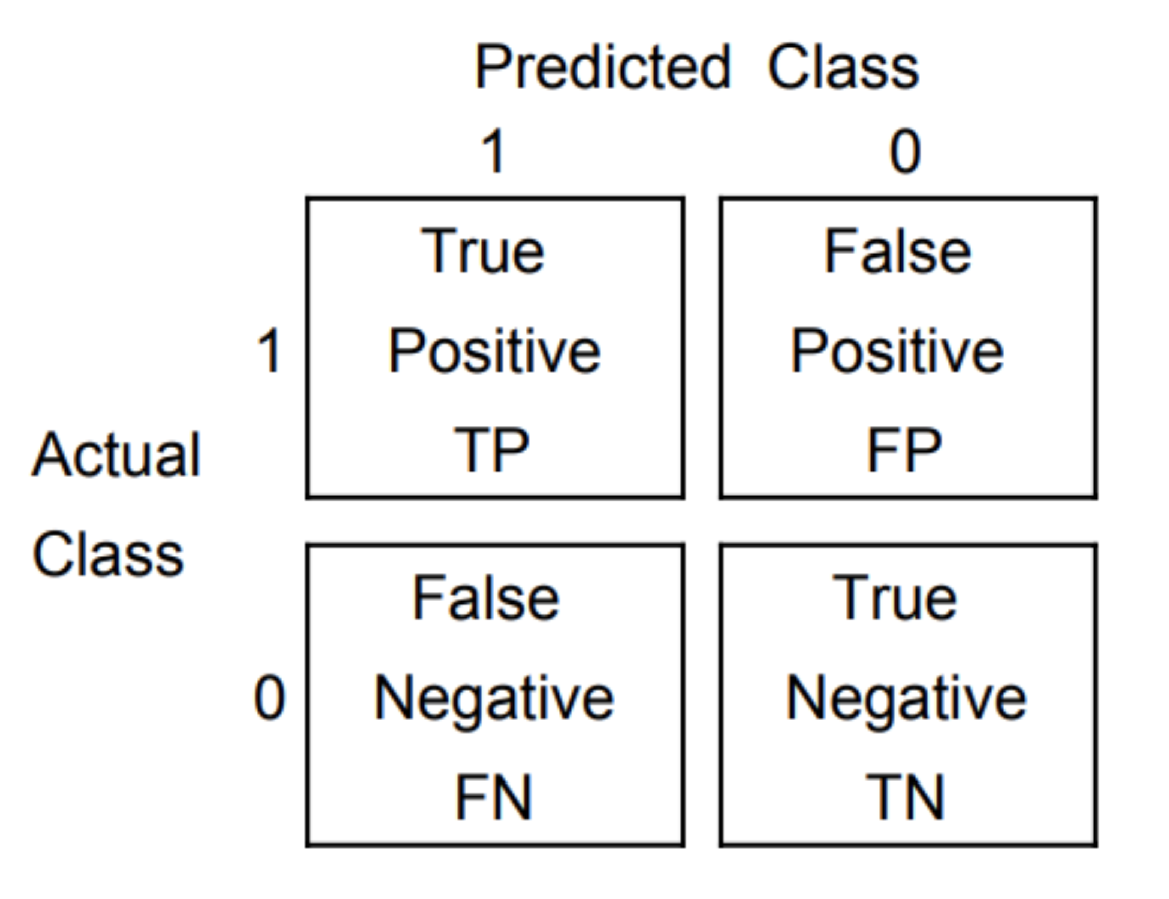
\includegraphics[scale=.5]{../Figures/Confuse_Mat_Example.png}\centering
\end{figure}

\subsection{Precision, Recall and F-Score}

Precision and Recall are two popular measurement to evaluate the performance of supervised classification methods. Precision is defined as:

$$\text { Precision } = \frac { True Postive } { True Postive + False Positive }$$

, recall defined as:

$$\text { Recall } = \frac { True Postive } { True Postive + False Negative }$$

and F-score is defined as the harmonic mean of both precision and recall:

$$F _ { 1 } = 2 \cdot \frac { \text { precision } \cdot \text { recall } } { \text { precision } + \text { recall } }$$

A classifier with high precision means it classifies almost no inputs as positive unless they are positive. A classifier high recall, on the other hand, would mean that the it misses almost no positive values. 
\section{Conclusion}

In this chapter, we briefly introduced some fundamental topics of Machine Learning theory required for natural language processing supervised classification tasks. We discussed two commonly used numerical methods to represent text computationally and their variants, Frequency-based methods: Bag-of word models (BoW) and Term Frequency - Inverse Document Frequency (tfidf), and Distributional similarity methods.In addition, we reviewed some techniques to reduce the dimensionality of feature space to reduce the complexity of the training and save computational resources. Finally, we covered how logistic regression as a probabilistic algorithm can be used for binary or multinomial classification along with the evaluation metrics used to gauge its performance. In the next two chapters, we will examine the use of multinomial logisitic regression classifier on two novel tasks in natural language processing: grammatical difficulty categorization of English sentences and automatic reading comprehension. We also explore how logisitic regression can be used in a semi-supervised manner to work on tasks with scarce data. 
% Chapter Template

\chapter{Theory} % Main chapter title

\label{Chapter2} % Change X to a consecutive number; for referencing this chapter elsewhere, use \ref{ChapterX}

%----------------------------------------------------------------------------------------
%    SECTION 1
%----------------------------------------------------------------------------------------

\section{Introduction} 

In this chapter, we explain the fundamentals of machine learning theory, with emphasis on supervised classification tasks. We start by describing the three primary stages of the machine learning process: feature extraction, classifier training, and testing and evaluation. We also discuss two types of feature engineering methods: frequency-based and distributional in addition to dimensionality reduction methods. Next, we introduce a linear classification technique called logistic regression and explain its mathematical foundations. Finally, we discuss the metrics used to evaluate the performance of supervised classification tasks.  

%Computers do not understand human language the way we do; they are limited by their innate nature of numerical computation. So in order to make use of decades worth of linguistic theories in the field of human language technology, tremendous human efforts must be extended to represent linguistic phenomena in a way computers are able to deal with. The goal is to unify the representation of textual documents
%whatever their formats by transforming them into a set of terms
%(features) that can be easily used by learning algorithms. Features can be thought of as any rule a linguist devises to represent particular characteristic of language. For instance, the presence of the substring `win \$1000 by clicking here` in an email may indicate for its spamminess. Feature engineering and design is an active research area in natural language processing, and its methods spans between manual and automatic creation.
%
%In order to apply learning algorithms on text, it is necessary to create
%a numerical representation of the text and assign a weight to each
%feature in text. This weighting is extremely important as it will
%influence the results of learning algorithms. Thus, a second objective
%is to improve weight the features.
%
%The number of features is a very important factor on which the
%performance of Text Classification depends. Indeed, several learning
%algorithms are unable to handle a large number of features. For this
%purpose, it is necessary to reduce the dimensionality of the
%representation space by keeping only the best features. Reduction
%methods are used to select or extract the most important features. In
%this chapter, we present most common automatic methods of text
%representation, specifying their advantages and disadvantages, and then we
%discuss the weighting techniques most used in Text Classification as
%well as the techniques used to reduce dimensionality.

\section{Classification as a Machine Learning Task}
Generally, there are two types of supervised learning tasks according to the data type of the predicted output: regression and classification. When the predicted output is a continuous value, such as predicting the price of a house or the temperature, the task is called regression. A classification task, on the other hand, is when the predicted output is a discrete value such as predicting the sentiment of a document (negative or positive) or predicting the weather state (rainy, sunny, cloudy, etc). 

The goal of a classification task is to select a correct class for a given input, or more generally a task of \enquote{assigning objects from a universe to two or more classes or categories} \citet[][p.575]{manning1999foundations}. A classifier is an algorithm that quantitatively models the relationship between a set of inputs and their associated outputs such that it learns how to label new data. In the task of spam filtering, for instance, input data are texts and the output are binary labels (0 or 1) representing whether or not a document is spam. 

Any classification task has two main phases: training and prediction ~\ref{fig:mlpipeline}. During training, a feature extractor is used to convert each input into a set of features which are designed to capture the basic information about each input. Next, pairs of feature sets and their corresponding labels are fed into the machine learning algorithm to generate a model. In the prediction phase, the trained model is used on unseen data to predict the labels. 

\begin{figure}
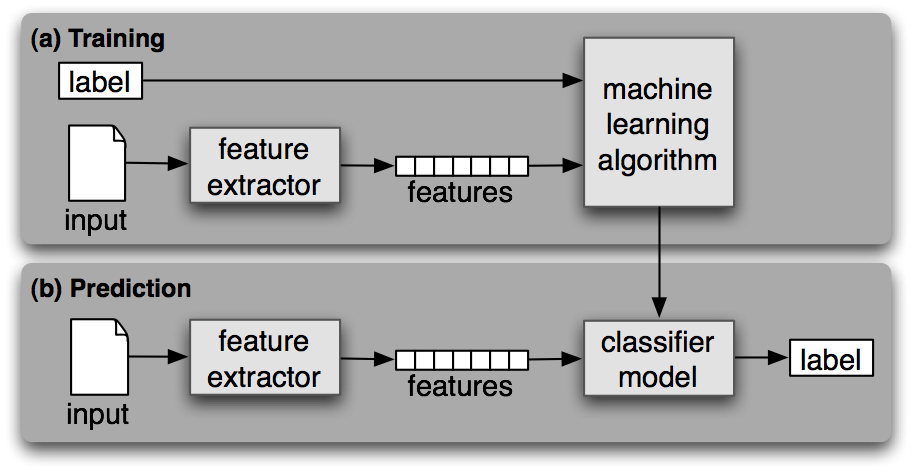
\includegraphics[scale=.8]{../Figures/mlpipeline.png} \centering
%\caption{\label{fig:mlpipeline}A diagram illustrating the pipeline of supervised classification learning, adopted from \protect\citeA[p.~222]{bird2009natural}}

\caption[Supervised Classification Learning Workflow]{A diagram illustrating the process of supervised classification learning, adopted from ~\citep[p.~222]{bird2009natural}}
\label{fig:mlpipeline}
\end{figure}

\section{Feature Extraction}

The first step in any machine learning task is feature extraction where a text input is transformed into a set of attributes that characterize it. One example of a negative sentiment document feature may be the presence of the word \emph{terrible}. Choosing what features to use when representing a text or a document not only has a major impact on the entire classification process, but it is also arguably the most difficult phase in any natural language processing task due to several fundamental questions on how do we represent language computationally. For example, on what level should we represent a text: \emph{character-wise}, \emph{word-wise} or \emph{sentence-wise}, or even more specifically morphologically, etymologically, or phonologically? Do we treat a word e.g. \emph{try} and all its morphological variations e.g. \emph{tries}, \emph{trying}, \emph{tried} similarly or differently? How to represent and model the semantics of human language computationally? Questions like these and many others are the core of natural language processing. Nevertheless, several automatic feature extraction methods have developed over the past decades that can be categorized into frequency-based or distributional, and we briefly explore some of the most common ones.

\subsection{Frequency-based Methods}

Frequency-based methods such as Bag-of-Words (BOW) and Term Frequency Inverse Document Frequency (TF-IDF) rely on the number of token occurrences in the text. They have been used extensively in a wide range of NLP applications, and each of them has advantages and disadvantages. 
% Representing a text computationally requires decision-making from the feature designer due to the complicated nature of human langauge language. 
\subsubsection*{Bag-of-Words Representation}

The bag-of-words (BOW) representation is the most straightforward and most intuitive
representation. It represents each document by a vector
whose component corresponds to the number of occurrences of a word in
the document.  To illustrate, the BOW vector representations of a data set of two documents (1) and (2) are shown in table \ref{tb:bow}:

\begin{enumerate}
\item The apple is better than the orange.
\item Summer is better than winter. 
\end{enumerate}




\begin{table}
\centering
\caption {Bag-of-words feature example}
\begin{tabular}{l|l|l|l|l|l|l|l|l|l|l}
 & the & apple & is & better & than & orange & summer & winter \\
Vector 1 & 2 & 1 & 1 & 1 & 1 & 1 & 0 & 0 \\
Vector 2 & 0 & 0 & 1 & 1 & 1 & 0 & 1 & 1 \\
\end{tabular}
\label {tb:bow}
\end{table}


Despite the simplicity of the BOW method,  it has two main disadvantages. One major disadvantage is that the BOW method pays no respect to the order of tokens in the document, and this can give similar representations to semantically different documents. For instance, the sentences \emph{The wolf eats the goat} and \emph{The goat eats the wolf} have similar vector representation , for they contain the exact same words. Another downside to BOW is that high frequency features are more important than low frequency ones. We can see in \ref{tb:bow} that the component corresponding to the first dimension (the) of vector 1 is bigger than in that of vector 2 because document 1 has two occurrence of the word \emph{the} while the document 2 has only one occurrence. 

To address the problem of order, several studies have attempted to count the occurrence of sentences instead of words \citep{fuhr1991probabilistic, tzeras1993automatic}. Although the sentences offer the advantage of better preserving the semantic relationship of the words, their use as features failed in practice. According to Lewis \citeyear{lewis1992representation}, this representation is penalized by a large number of possible combinations which leads to low and highly
random frequencies. A more practical approach is representation by n-grams. It consists of breaking the text into moving sequences of $n$ consecutive tokens. For example, the trigram segmentation of the word "language" gives the following 3-grams: lan, ang, ngu, gua, uag, age. \citep{shannon1948mathematical}, who was interested in predicting the appearance of certain characters according to the other characters introduced the notion of n-grams. Since then, n-grams have been used in many areas such as speech recognition and information retrieval. Using n-gram on a character-level or word-level gives a contextual representation of the text. A modification to BOW to overcome the bias of high frequency tokens resulted in devising a method called Term Frequency Inverse Document Frequency (TF-IDF). 

\subsubsection*{TF-IDF Representation}

TF-IDF has two main parts. Term Frequency is proportional to the frequency of the term in the document (local weighting)and can be used as is or in several variations \citep{sable2001using, singhal1997learning}.

$$t f _ { i j } = f \left( t _ { i } , d _ { j } \right)$$

$$t f _ { i j } = 1 + \log \left( f \left( t _ { i } , d _ { j } \right) \right)$$

$$ t f _ { i j } = 0.5 + 0.5 \frac { f \left( t _ { i } , d _ { j } \right) } { m a x _ { t _ { i } \in d _ { j } } f \left( t _ { i } , d _ { j } \right) }$$

where $f(t_{i},d_{j})$ is the term frequency of document $j$. Variations include logarithmic scaling of frequency counting or normalization. 

Inverse Document Frequency (IDF) measures the importance of a term throughout the collection (overall weighting). A term that often appears in the document base should not have the same impact as a less frequent term. Indeed, terms that appear in the majority of documents do not have any discriminating power to distinguish documents from each other and must, therefore, have low weightings. The IDF weighting is inversely proportional to the number of documents containing the term to be weighted. Thus, the more the term appears in several documents, the less it is discriminating, which results in being assigned a low weighting. The IDF weighting is generally expressed as follows:

$$i d f \left( t _ { i } \right) = \log \left( \frac { N } { d f \left( t _ { i } \right) } \right)$$

where $df(t_{i})$ is the term frequency of feature $i$ and $N$ is the number of documents in the corpus.

The TF-IDF weighting combines the two weightings, TF and IDF, in order to
provide a better approximation of the importance of a term in a
document. According to this weighting, for a term to be important in a
document, it must frequently appear in the document but rarely occur in other
documents. This weighting is given by the product of the term's local weighting
in the document by its overall weighting in all the
documents of the corpus.

$$t f i d f \left( t _ { i } , d _ { j } \right) = t f _ { i j } \times \log \left( \frac { N } { d f \left( t _ { i } \right) } \right)$$

Frequency-based text representation methods explored so far, despite their usefulness in a variety of tasks in natural language processing, share sparsity as one problem in common. The number of features generated using these methods can easily exceed the tens of thousands, which not only negatively influences the categorization process, but it is also very computationally expensive in terms of hardware resources. In addition, the higher the dimensions of the features are, the weaker the features become. This problem is known as the \emph{curse of dimensionality} \citep{bellman2015adaptive}. To remedy this issue,  techniques borrowed from the field of information theory and linear algebra have been developed to reduce the feature space dimensionality without losing much information. 
% Frequency-based representation emthods, in both of its variants BOW and tfidf, drive most of search engines and recomednation systems algorithms, but they still share a critical problem of sparsity. The number of features of a data set is equal to the union of all terms in the data set, and this can be extremely large in size. Therefore, we will explore some techniques to address this issue.  
% TFC is a modification to TFIDF that overcomes the major drawback of the
% TFIDF measure, namely that the length of the documents is not taken into
% consideration by adding a normalization factor. The TFC weighting of a
% term $i$ in a document $j$ is calculated as follows:

% $$T F C _ { i j } = \frac { T F I D F \left( t _ { i } , d _ { j } \right) } { \sqrt { \sum _ { k = 1 } ^ { T } T F I D F \left( t _ { k } , d _ { j } \right) ^ { 2 } } }$$
% The use of n-grams offers the following advantages: 1) language-independent 2) Requiring no prior segmentation of the document. 3) Less sensitive to misspellings. 4) effective method to automatic language identification.

% The first challenge is how to identify words. In English, for instance, while white-space character is the indicator of words boundry, there are cases like \emph{New York} that need decision on whether or not they should be treated as one or two words. A word as being a sequence of
% characters belonging to a dictionary, or formally, as being a sequence
% of characters separated by spaces or punctuation characters. This
% definition is not valid for all languages. Indeed, languages such as
% Chinese or Japanese do not separate their words by spaces. In addition, some separators can be part of certain words (for example today,
% 127.0.0.1, potato). Another difficulty concerns the management of
% compound words (for example rainbow, potato) and acronyms (like:
% IBM, CAF, CAN, etc.). Consideration of these cases requires quite
% complex language treatments. This representation of texts excludes any
% grammatical analysis, and any notion of order between words and therefore
% semantically distant texts can have the same representation. For
% example, the sentences \texttt{the\ wolf\ eats\ the\ goat} and
% \texttt{the\ goat\ eats\ the\ wolf} is given the same representation
% despite being semantically different.

% \subsubsection{Representation by Sentences}

% Bag-of-words representation excludes any notion of order and
% the relationship between the words of a text, several studies have
% attempted to use sentences as features instead of words \citep{fuhr1991probabilistic} \citep{tzeras1993automatic}.
% The use of the sentences makes it possible to solve the problem of
% ambiguity generated by the use of the representation "bag of words." For
% example, the word \texttt{mouse} has several possible meanings while
% optical mouse and domestic mouse has no ambiguity. Although the
% sentences have the advantage of better keeping the semantics in relation
% to the words, their use as features did not lead to the expected
% results. According to Lewis \citep{lewis1992representation}, this representation is penalized
% by a large number of possible combinations which leads to low and too
% random frequencies. One solution proposed in \citep{caropreso2001learner} was to consider a
% sentence as a set of contiguous (but not necessarily ordered) words that
% appear together but do not necessarily respect grammatical rules.

% \subsubsection{Representation by lemmas or lexical roots}

% A modification to the "bag of words" is representation by lemmas or lexical roots which replaces  each word by its canonical form so that words with different
% forms (singular, plural, masculine, feminine, present, past,
% future) can have in a single form called a canonical form.
% Grouping the different forms of a word offer the advantage of reducing the dimensionality of the learning space. Indeed, in the bag-of-words representation, each form of a word is given a dimension; while with lemma representation the different forms of one word will be merged into one dimension. For example, words such as play, player, players, plays, and played will be replaced by the lemma play.


% Lemmatization and stemming are the two techniques used to find the canonical form of a word. Lemmatization uses a knowledge base containing the different inflected forms corresponding to the different possible lemmas. Thus, the inflected forms of a noun will be replaced by the singular masculine form while the infinitive form will replace the different inflected forms of a verb. Lemmatization requires the use of a dictionary of inflected forms of language as well as a grammar labeler. An efficient algorithm, named TreeTagger \citep{schmid1994probabilistic}, has been developed for thirteen different languages: German, English, French, Italian, Dutch, Spanish, Bulgarian, Russian, Greek, French Portuguese, Chinese, Swahili, and Old French. Stemming uses a knowledge base of syntactic and morphological rules and to transform words into their roots. One of the most well-known stemming algorithms for the English language is Porter's algorithm \citep{porter1980algorithm}. Lemmatization is more complicated to implement since it depends on the grammatical labelers. In addition, it is more sensitive to misspellings than stemming.

% \begin{lstlisting}[language=Python, caption=Python example]
% def stem(word):
%     Suffix_list = ["ing","ly","ed","ious",\
%                 "ies","ive","es","s","ment"]
%     for suffix in Suffix_list:
%         if word.endswith(suffix):
%             return word[:-len(suffix)]
%     return word
% \end{lstlisting}

% \subsubsection{Representation by n-grams}




% \subsubsection{Representation by concepts}



% \subsubsection{Weighting of the features}

% Co-occurrence methods such as bag-of-words have significant drawbacks, one of which is terms with higher frequency are more important than those with less frequency. Several normalization methods were developed to remove the bias towards more frequent terms. One of these methods is Term Frequency Inverse Document Frequency (TFIDF).



\subsection{Dimensionality reduction}

There are a number of linguistic and non-linguistic ways to reduce the number of features in text data. Depending on the task, we can aggregate words of certain linguistic relation in concepts. For example, we replace co-hyponyms \emph{dog} and \emph{wolf} with their hypernym \emph{canine}; or \emph{vehicle} and \emph{car} with \emph{automobile}. Concepts, defined as units of knowledge, can be used as features to solve the ambiguity problem as well as the problem of synonymy. Indeed, each concept represents a unique meaning that can be expressed by several synonymous words. Similarly, a word with many meanings (senses) is found mapped to several concepts. Thus, a document containing the word \emph{vehicle} may be indexed by other words, such as car or automobile. The transition from a word representation to a concept representation requires the use of semantic resources external to the content of documents such as semantic networks, thesauri, and ontologies. As a result, the performance of such a representation crucially depends on the semantic richness of the resources used in terms of the number of concepts and relationships between these concepts. 

In some cases, we may need to treat morphologically variant words similarly. For example, words such as play, player, players, plays, and played will be replaced by \emph{play}. Lemmatization and stemming are the two techniques used to find the canonical form of a word. Lemmatization uses a knowledge base containing the different inflected forms corresponding to the different possible lemmas. Thus, the inflected forms of a noun will be replaced by the singular masculine form while the infinitive form will replace the different inflected forms of a verb. Lemmatization requires the use of a dictionary of inflected forms of language as well as a grammar labeler. Stemming uses a knowledge base of syntactic and morphological rules and to transform words into their roots. One of the most well-known stemming algorithms for the English language is Porter's algorithm \citep{porter1980algorithm}. Lemmatization is more complicated to implement since it depends on the grammatical labelers. In addition, it is more sensitive to misspellings than stemming.

\begin{lstlisting}[language=Python, caption=An example of simple Stemmer Written in Python]
def stem(word):
    Suffix_list = ["ing","ly","ed","ious",\
                "ies","ive","es","s","ment"]
    for suffix in Suffix_list:
        if word.endswith(suffix):
            return word[:-len(suffix)]
    return word
\end{lstlisting}

Dimensionality reduction can also be done using probabilistic and linear algebraic techniques such as principal component analysis (PCA) and linear discriminant analysis (LDA) that aim to project highly dimensional data into lower dimension space. However, we limit the discussion to only two methods: clustering and Latent Semantic Allocation. 

Clustering \citep{baker1998distributional, sable2001using, slonim2001power} can be used to reduce dimensionality. It consists of representing the documents in a new representation space other than the original one — each dimension of the new representation space groups terms that share the same meaning. Thus, the documents will no longer be represented by terms but rather by groupings of terms representing semantic concepts. This new space of representation offers the advantage of managing the synonymy since the synonymous terms will appear in the same groupings. Likewise, the fact that a term can be included in several groupings also makes it possible to manage the polysemy. Another exciting method to reduce dimensionality, proposed by \cite{deerwester1990indexing} is Latent Semantic Allocation (LSA). It uses singular value decomposition of the document's $x$ term matrix to change the representation by keeping only the $k$ axes of the strongest singular values. However, LSA is very expensive in terms of calculation time during learning as it relies on a matrix factorization method called Singular Value Decomposition (SVD), which runs computationally in cubic size. Likewise, with each new document, it is necessary to redo the whole grouping process.

\subsection{Distributional Method}
An alternative approach for text representation in natural language of processing is the distributional similarity, which represents the meaning of a word using words that co-occur in the same context. For example, the words 'dog' and 'cat' have the same meaning in the following two sentences: \emph{I have a cat}; \emph{I have a dog}. While this idea might not be adequate to capture or account for the complexity or the sophistication of human language, it has succeeded tremendously in a variety of lexicalized NLP tasks. It has become the de facto representation method of text. The need for such a method does not only come from the need for more accurate numerical representation, but its density compared to other methods makes it less computationally expensive. Word2Vec \citep{mikolov2013distributed} and GloVe \citep{pennington2014glove} are two famous algorithms for creating word embedding. 

The intuition of word2vec is to train a classifier on a binary prediction task: “Is
word $w$ likely to show up near X?”, where $X$ is the word to which we want to find embeddings. Then, we use the weights learned by the classifier as embeddings. Skip-gram algorithm \citep{mikolov2013distributed} , first, initializes embeddings randomly. Then, it iteratively updates the embeddings of each word $w$ to be equal to the words they occur within the same context. Finally, it injects a, $k$, number of non-neighbor words as negative examples. 

\section{Logistic Regression}

Logistic regression is a machine learning classifier that is used for a variety of learning tasks in natural language processing and image processing. It belongs to a group of probabilistic classifiers called discriminative models which, unlike its generative counterparts like Naive Bayes classifiers, tries to distinguish the classes rather than learn to generate them. More formally, given a document, $x$, and a class $y$, a logistic regression classifier computes the conditional probability of a class, $y_i$, given its input $x_i$ $P(y|x)$. There are two types of logistic regression classifiers: binary and multinomial. The binary logisitc regression is used when there are two classes of inputs to be predicted such as spam or not spam; positive or negative; malignant or benign. Multinomial or multi-class logistic regression is used when there are more than two predicted classes, such positive, neutral, or negative.

 According to \cite{jurafsky2014speech}, classification using logistic regression, like any other supervised classification algorithm, has four main components: 

\begin{list}{•}{}
 \item a feature extractor, which  numerically represents language data (characters, words and sentences, etc) input, $\mathbf{X}$, as feature vector $\left[x_1,x_2,\ldots,x_n \right]^T$ where $n$  represents the number of features in the input data;

\item a classification function to compute an estimation to class $\hat{y}$ via $p(y|x)$ and determine whether the classifier is binary or multinomial; 
 
\item an objective function to minimize the error predicted label $\hat{y}$ and actual label, $y$, in training examples (cross entropy); and

\item an optimizer to help find the minimum of the objective function 
 (stochastic gradient descent).
 \end{list}

% Logistic regression also has two phases: training and testing. In the training phase, the goal is to find the optimal weights that best account for mapping input features $x_{i}$ to the labeled output $y_{i}$ of a subset of the data. In testing, we measure the generalizability of weights learned in the training phase on the remaining set of the data.

% Formally, the goal of logisitic regression is to learn the set of weights $\theta$ that minimizes the loss between the true $y$ labels in the training data given the input data $x$
Given a dataset of $m$, number of observations, $x$, and classes, $y$, $\mathcal { D } = \left\{ \left( \boldsymbol { x } ^ { ( i ) } , y ^ { ( i ) } \right) \right\} _ { i = 1 } ^ { m }$, the goal is to learn the set of optimal weights $\hat{w}$ that maximizes the log probability of predicting a class, $y$, given an observation, $x$

\begin{equation}
\hat{w}=\underset{w}{\operatorname{argmax}}\left[\sum_{1=i}^{m} \log P\left(y^{(i)} | x^{(i)}\right)\right]
\end{equation}

The distribution type of $P\left(y^{(i)} | x^{(i)}\right)$ determines whether the type of learning is binary or multiclass. The probability distribution of binary output is Bernoulli, while the probability distribution of multiclass output is multinomial. 

\subsection{Classification Functions}
What we have discussed so far gives us a method to numerically translate language from a form that is uniquely comprehensible to humans into a representation that a computer can understand, and can somehow capture the characteristics of human language. However, in order for the logistic regression to learn to classify, a classification function should be utilized. Depending on whether the classification task is binary or multinomial, there are two main functions used: Sigmoid and Softmax. Sigmoid function, used for binary classification, outputs 1 if an observation input (feature vector) is a member of a particular class e.g. (spam), and 0 otherwise. In other words, it calculates $P(y=1|x)$ for spam text and $P(y=0|x)$ for non-spam text. The mathematical form of the Sigmoid function or (logistic function, hence comes the name of the classifier) is as follows:

$$Sig ( x ) = \frac { 1 } { 1 + e ^ { - (w \cdot x +b)} }$$ 

where $x$ represent the input vector, $w$ is the learned weights, and $b$ is the bias term or the intercept of the linear equation. One mathematical property of the Sigmoid function is that it maps any input between 0 and 1, and to make it as probability we need to make the sum of $P(y=1)$ and $P(y=0)$ equals to 1. 

$$ P ( y = 1 ) = \sigma ( w \cdot x + b ) $$
$$ P ( y = 0 ) = 1 - \sigma ( w \cdot x + b ) $$

The classifier declares an observation input as \emph{Yes} (if it is a member of class spam) if the probability is greater than a certain threshold, say 0.5, and declares an observation input as \emph{No} otherwise. 

$$  \hat { y } = \left\{ \begin{array} { l l } { 1 } & { \text { if } P ( y = 1 | x ) > 0.5 } \\ { 0 } & { \text { otherwise } } \end{array} \right.  $$


In the case of multinomial classification, the logic remains the same except for the classification function where Softmax is used rather than Sigmoid. Softmax works on normalizing the prediction of an observation by the values of all other classes in order to produce valid probability distribution. 

$$p ( y = i | x ) = \frac { e ^ { w _ { i } \cdot x + b _ { i } } } { \sum _ { j = 1 } ^ { k } e ^ { w _ { j } \cdot x + b _ { j } } }$$



\subsection{Objective Functions}

During the learning process, we need to answer the question, \emph{how correct is the estimated output of $\hat{y}$ of classifier from the true output $y$?}. Therefore, our objective \emph{function} is to minimize the difference between the estimated output and the true one such that the weights learned during this minimization process are, hopefully,  generalizable enough to correctly label observations unseen in the training phase. We can imagine an objective function to be the difference between the $\hat{y}$ and $y$ i.e. $\left | \hat{y} - y \right |$, but for mathematical convenience we need a non-convex objective function that can be easily optimized. Thus, we use maximum likelihood estimation. 

Binary classification can be seen as Bernoulli distribution since the outcome is either 0 or 1. More formally, the probability of predicting class $y$ given input $x$ is  $p ( y | x ) = \hat { y } ^ { y } ( 1 - \hat { y } ) ^ { 1 - y }$. Minimizing the probability is the same as maximizing the negative log likelihood:
 $$L _ { C E } ( \hat { y } , y ) = - \log p ( y | x ) = - [ y \log \hat { y } + ( 1 - y ) \log ( 1 - \hat { y } ) ]$$

Finally, by plugging in the value of $\hat{y}$ we obtain:
$$ L _ { C E } ( w , b ) = - \frac { 1 } { m } \sum _ { i = 1 } ^ { m } y ^ { ( i ) } \log \sigma \left( w \cdot x ^ { ( i ) } + b \right) + \left( 1 - y ^ { ( i ) } \right) \log \left( 1 - \sigma \left( w \cdot x ^ { ( i ) } + b \right) \right) $$, where $m$ is the number of training examples.

On the other hand, multinomial classification uses the same process except that it uses a different classification function softmax and hence has different (multinomial) distribution. As a result, the loss function for a single example $x$ is the sum of the logs of the $K$ output classes:
$$ L _ { C E } ( \hat { y } , y ) = - \sum _ { k = 1 } ^ { K } 1 \{ y = k \} \log \frac { e ^ { w _ { k } \cdot x + b _ { k } } } { \sum _ { j = 1 } ^ { K } e ^ { w _ { j } \cdot x + b _ { j } } } $$

\subsection{Optimization}

The objective functions derived in the previous section is optimized using numerical methods. Several algorithms are used for this purpose, such as Stochastic Gradient Descent, which uses first derivative (gradient) information to find a minimum of a function, and Newton-Raphson algorithm, which uses Second derivative information to find a minimum of a function. Discussing the details of how these algorithms work and the mathematical derivation of gradients is beyond the scope of this work. (See \citep{jurafsky2014speech} for more details on the derivation of Stochastic Gradient Descent.) 

\section{Evaluation Metrics}
\subsection{Confusion Matrix}

A confusion matrix is a method to visualize the results of a classification algorithm. For the binary classification, the algorithm can be used to predict whether a test sample is either 0, or 1. As a way to measure how well the algorithm performs, we can count four different metrics, where 1 defined as positive and 0 is defined as negative:

\begin{enumerate}

\item True positive (TP), the algorithm classifies 1, where the correct class is 1.
\item False positive (FP), the algorithm classifies 1, where the correct class is 0.
\item True negative (TN), the algorithm classifies 0, where the correct class is 0.
\item False negative (FN), the algorithm classifies 0, where the correct class is 1.

\end{enumerate}

\begin{figure}[hbtp]
\caption{Confusion Matrix Example}
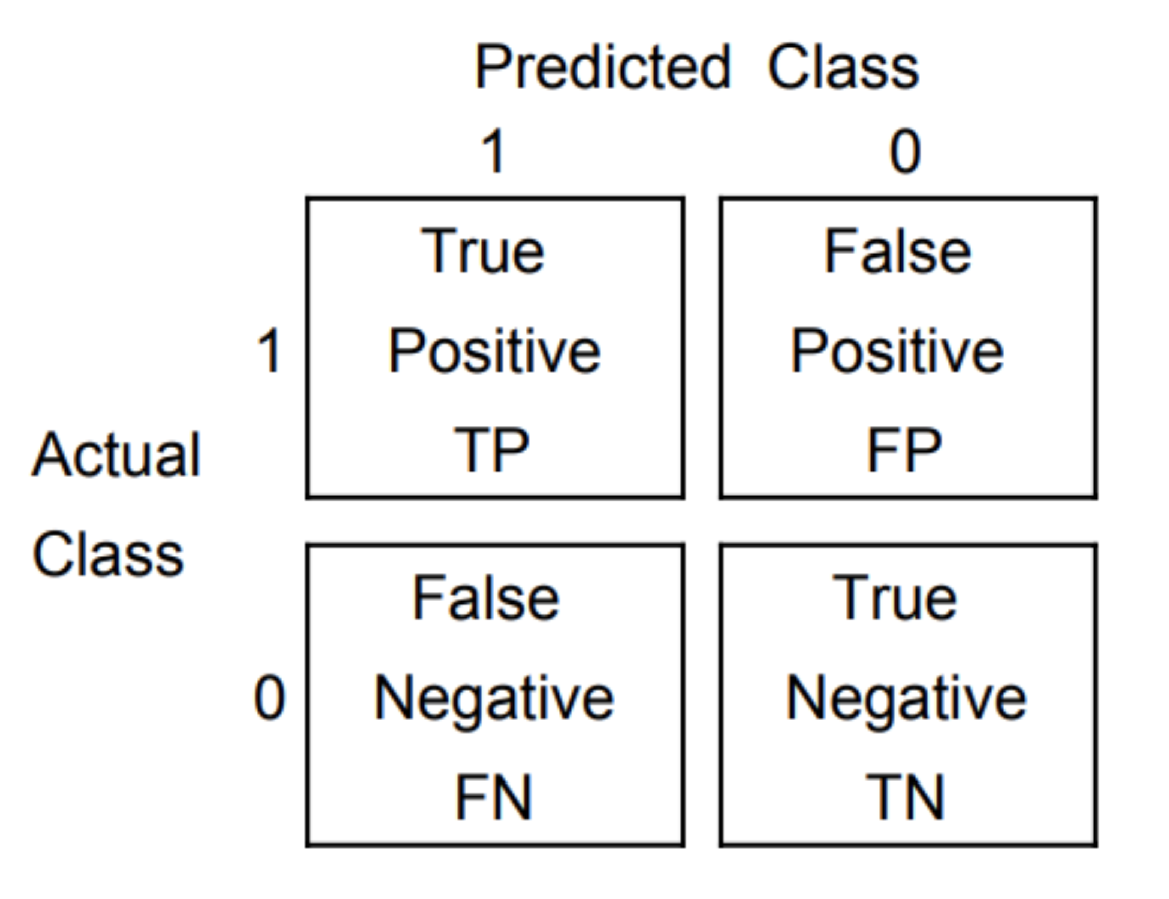
\includegraphics[scale=.5]{../Figures/Confuse_Mat_Example.png}\centering
\end{figure}

\subsection{Precision, Recall, and F-Score}

Precision and Recall are two popular measurements used to evaluate the performance of supervised classification methods. Precision is defined as follows:

$$\text { Precision } = \frac { True Postive } { True Postive + False Positive }$$

; Recall is defined as:

$$\text { Recall } = \frac { True Postive } { True Postive + False Negative }$$

and F-score is the harmonic mean of both precision and recall:

$$F _ { 1 } = 2 \cdot \frac { \text { precision } \cdot \text { recall } } { \text { precision } + \text { recall } }$$

A classifier with high precision means it classifies almost no inputs as positive unless they are positive. A classifier with high recall, on the other hand, would mean that  it misses almost no positive values. 
\section{Conclusion}

In this chapter, we briefly introduced some fundamental topics of Machine Learning theory required for natural language processing supervised classification tasks. We discussed commonly used feature extraction methods, such as BOW, TF-IDF, and Distributional similarity. Additionally, we reviewed some techniques to reduce the dimensionality of feature space to reduce the complexity of the training and save computational resources. Finally, we discussed how logistic regression as a probabilistic algorithm can be used for binary or multinomial classification along with the evaluation metrics used to gauge its performance. In the next two chapters, we show the use of multinomial logistic regression classifiers on two novel tasks in natural language processing: grammatical difficulty categorization of English sentences and automatic reading comprehension. We also explore how logistic regression can be used in a semi-supervised manner to work on NLP tasks with limited data.  
% Chapter Template

\chapter{Two-stage Classifcation Method for Automatic Reading Comprehension } % Main chapter title

\label{Chapter3} % Change X to a consecutive number; for referencing this chapter elsewhere, use \ref{ChapterX}

\section{Introduction}

Machine Comprehension or Automatic Reading Comprehension is the task of automatically answering comprehension questions based on information derived from short texts. While this task is relatively easy for the humans to do, it is hard for the machine because it requires not only linguistic information, but also cognitive, world-knowledge skills as well. Machine Comprehension has been of great interest to NLP community because of its practical applications in education, especially in the field of automated assessment and intelligent tutoring systems. Working on similar tasks will bring us a step closer to understand how human is able to perform such cognitive tasks so easily while machine is not. \\

In this chapter, we will be using the second release of Stanford Question Answering Dataset (SQuAD) \citep{rajpurkar2018know}. SQuAD 2.0 is a reading comprehension dataset, consisting of 150K questions posed by crowdworkers on a set of Wikipedia articles, where the answer to every question is a segment of text, or span, from the corresponding reading passage, or the question might be unanswerable. The difference between SQuAD 2.0 and its previous release is that it has 50K unanswerable questions in addition to paragraph-supported questions.  To do well on SQuAD2.0, a system must not only answer questions when possible, but also abstain from answering when no answer is supported by the paragraph. \\

The strategy will be used to tackle this task is mainly driven by a simple linguistic intuition. Since SQUAD 2.0 task is an  question answering task, the answer span lies within one of given sentences in the paragraph, then an answer is one of the constituents of the best candidate sentence. Thus, our goal is to, first, find the sentence containing the right answer, and we do by training a logistic regression classifier with some linguistic features. Then, we train another classifier to find the constituent best represent the right answer span within the sentence predicted in the first stage. In order to account for the unanswerability of some of the questions, we add a null-answer as a dedicated class in the first classifier along with the potential sentences. This way, if an answer is not found, the inference process stops without proceeding to the next stage, which saves time and computation. 



\section{Related Work}

There has been a large number of studies tackle traditional Machine Comprehension tasks, where answers are extractive and explicitly stated in the passage. The difficulty of SQUAD 2.0 task, however, lies in abstaining from answers when no answer span exist in the passage. Thus, we will focus on models that not only answers the questions, but also the one that predict the probability of questions being answered.  


\citep{DBLP:journals/corr/SeoKFH16} introduced bi-directional attention flow (BiDAF) that uses an recurrent neural network to encode contextual information in both question and passage along with an attention mechanism to align parts of question to the sentence containing the answer and vise versa. The model offers context representation at multilevel of granularity: character-level, word-level and contextual embedding. What sets this work from others is that it does not represent the context paragraph into fixed-length vector. Instead, it dynamically computes vectors at each time step, combines it with the one from previous layer and allow \textit{flow} through to the next layers. The model outputs confidence scores of start and end index of all potential answers. One problem with this model is it is not designed to handle unanswerable questions. \citep{DBLP:journals/corr/LevySCZ17} extends the work by assigning a probability to null-answers to account for the questions whose answers do not exist in the corresponding paragraph. It achieves 59.2\% EM score and 62.1\% F1 score.\\

\citep{DBLP:journals/corr/abs-1808-05759} propose a read-then-verify system that is able to abstain from answering when a question has no answer given the passage. They introduce two auxiliary losses to help the neural reader network focus on answer extraction and no-answer detection respectively, and then utilize an answer verifier to validate the legitimacy of the predicted answer. One key contribution is answer-verification. The model incorporates multi-layer transformer decoder to recognize the textual entailment that support the answer in and passage. This model achieves an ExactMatch EM score of 71.6\% and 74.23\% F1 on SQuAD 2.0. \\

\citep{DBLP:journals/corr/abs-1811-11934} proposes a new hierarchical attention network that mimics the human process of answering reading comprehension tests. It gradually focuses attention on part of the passage containing the answer to the question. The modal comprises of three layers. a) \textbf{encoder layer}: builds representations to both the question and the passage using a concatenation of word-embedding representation \citep{pennington2014glove} and a pre-trained neural language modal \citep{Peters:2018} b) \textbf{Attention layer}: its function is to capture the relationship between the question and the passage at multiple levels using self-attention mechanisms. c) \textbf{Matching layer}: given refined representation for both question and passage, a bi-linear matching layer detects the best answer span for the question. This method achieves the state-of-the-art results as of September 2018. Their single model achieves 79.2\% EM and 86.6\% F1 score, while their ensemble model achieves 82.4\% EM and 88.6\% F1 Score. \\

Current models that have shown significant improvement on Machine Comprehension tasks and other similar ones owe their success to a recent neural architecture called transformer networks \citep{DBLP:journals/corr/VaswaniSPUJGKP17}. It has become the \emph{de facto} in recent sequential learning tasks, eschewing recurrence. This architecture creates global dependencies between input and output using only attention mechanisms. An even more successful model is Bidirectional Encoder Representations from Transformers BERT \citep{DBLP:journals/corr/abs-1810-04805}. It is a task-independent pretrained language model that uses a deep transformer network to create rich and context-specific vector representation. Using a method called Masked Language Model, the goal is to randomly mask tokens from the input and predict the vocabulary id of the masked word based only on its context. BERT has shown significant improvement on several tasks, one of which is SQUAD. 


While these models achieve astonishing results, they are  complex in terms of architecture design and implementation, and very resource-intensive. This complexity results due to  lack of linguistic assumptions that can arguably constrain and direct the problem. 

%The baseline for the task is a simple logistic regression with a set of features, and I would argue that adding more feature could achieve good results at a fracture of cost and complexity.

\section{Baseline Implementation}

The new version of SQuAD 2.0 task adds a new constraint to competing question-answering models. In addition to identifying  the extractive answer spans, a question-answering model should abstain from answering if the passage does not contain an answer. To this end, we implement a simple multinomial logistic regression classifier to address this task. At this level, the classification task is to predict the sentence, in the paragraph, containing the right answer, or declaring that the question is unanswerable. Next, we apply a constituency parser over the sentence predicted from the first stage to get its constituents among which lies the correct answer span (see Figure 1).  

\begin{figure}
  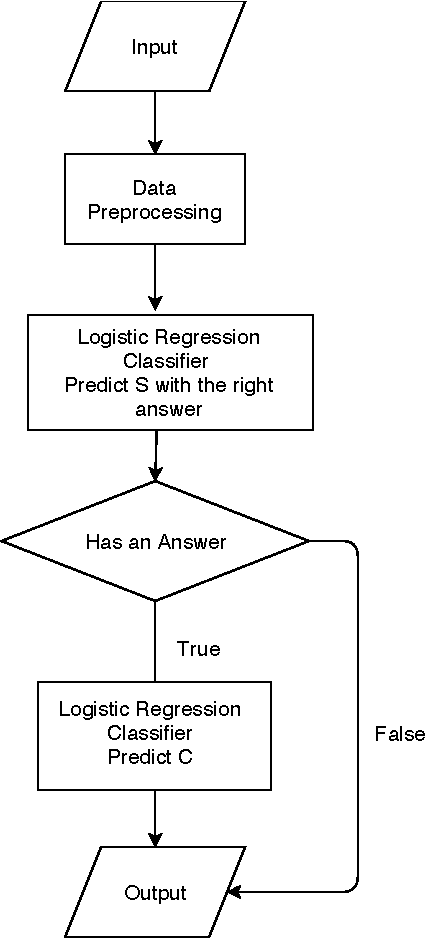
\includegraphics[scale=1]{../Figures/Flowchart.pdf}\centering
  \caption{Flowchart illustrating the two-stage classification approach}
\end{figure}


\subsection{Feature Design} 
To find the sentence containing the answer, a classifier must determine the sentence that is most similar to the question, and by similar we mean that a good candidate sentence  1) shares more words with the question. 2) has high cosine similarity with the question. 3) shares syntactic similarity with the question. Thus, three main features have been selected to this end:
\begin{itemize}
\item \textbf{Cosine Similarity}: for every sentence in the paragraph as well as the question a word vector representation is created via InferSent (Conneau et al, 2017), which is a pre-trained sentence embeddings method that provides semantic representations for English sentences. InferSent is an encoder based on a bi-directional LSTM architecture with max pooling, trained on the Stanford Natural Language Inference (SNLI) dataset. Cosine distance score is calculated for each sentence-question pair. 
\item \textbf{Word Overlap}: this calculates the Jaccard score between each sentence-question pair. Jaccard index is a method of computing the explicit similarity between two sets as follows: 
$$
J(Q,S) = \frac{|Q \cap S|}{|Q \cup S|}
$$
where Q and S are sets of words in question and sentence respectively.

\item \textbf{POS Overlap}: This feature computes the Jaccard score over the part-of-speech-tag representation of sentences. In other words, instead of the word tokens, it checks similarity over POS tokens.We use the default POS-tagger in the Spacy library of Python programming language to obtain the POS representation for the sentences and questions alike.
\end{itemize}
Using the three features above every question-sentence pair will have three scores and an additional binary feature indicating whether or not the question is answerable. This latter feature is provided by the dataset. 
\subsection{Training and Result} 
We train a logistic regression classifier with L2 regularization (`newton-cg' solver) using scikit-learn library of Python programming language, and we get the results shown in table 1. Numbers in class column represents the index of the sentence in paragraph containing the answer, and -1 indicates that the question has no answer in the paragraph. We also limit the number of sentence to 10. The results show that with simple features we get an F1 score of 0.71.

\begin{figure}
  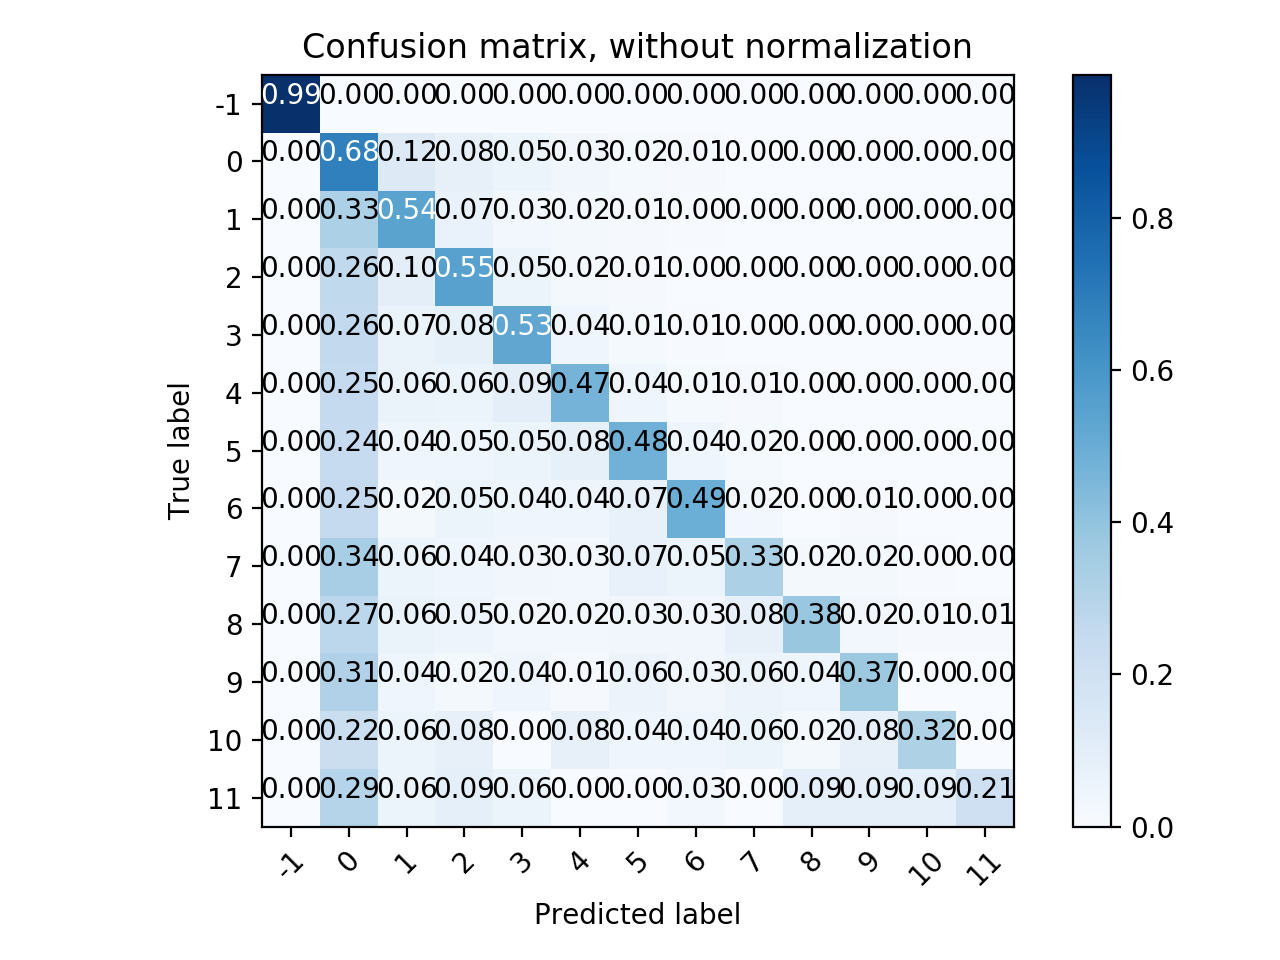
\includegraphics[scale=1]{Figure_1.png}\centering
  \caption{Confusion matrix shows which classes were predicted correctly}
\end{figure}

\begin{table}[]

\begin{tabular}{lllll}\centering
\hline \textbf{class} & \textbf{precision} & \textbf{recall} & \textbf{F1-score} \\ \hline

 -1	&	1	&	0.99	&	0.99		\\ 
0	&	0.47	&	0.68	&	0.56		\\
1	&	0.63	&	0.54	&	0.58	\\
2	&	0.62	&	0.55	&	0.58		\\
3	&	0.62	&	0.53	&	0.57		\\
4	&	0.58	&	0.47	&	0.52		\\
5	&	0.57	&	0.48	&	0.52		\\
6	&	0.57	&	0.49	&	0.53		\\
7	&	0.46	&	0.33	&	0.38	\\
8	&	0.56	&	0.38	&	0.45		\\
9	&	0.46	&	0.37	&	0.41		\\
10	&	0.48	&	0.32	&	0.39	\\
11	&	0.35	&	0.21	&	0.26		\\
\hline avg / total	&	0.72	&	0.71	&	0.71		\\ \hline

\end{tabular}
\caption{This table shows the results of running a multinomial regularized logistic regression. Class column represents the index of sentences within the paragraph, and -1 represent the unanswerable question case. Unpredicted classes are removed.}
\label{my-label}

\end{table}

\newpage

\section{Stage Two: Predicting the Answer Span}
\subsection{Iteration 1}
To select the most plausible answer span from the candidate sentence, we design a number of features:
\begin{itemize}
\item \textbf{Constituents}: Using a constituency parser \citep{kitaev2018constituency}, we obtain all constituents in a candidate sentence. These constituents will be the classes from which we pick the right span.
\item \textbf{Contextual Overlap}: Constituents sharing context with the original question are potential candidates to be the correct answers. So we measure the cosine similarity between each constituent and the question:
$${ similarity } = \frac { \sum _ { i = 1 } ^ { n } C _ { |w| } Q _ { i } } { \sqrt { \sum _ { i = 1 } ^ { n } C _ { |w| } ^ { 2 } } \sqrt { \sum _ { i = 1 } ^ { n } Q _ { i } ^ { 2 } } }$$ 
where $w$ is the number of slide window around the candidate constituent. For our purposes features of size 2 and 3 are used. 

\item \textbf{Constituent Label}: Constituency parse tree label of the span combined with wh-word.
\end{itemize}
Out of 85K training example, the answer spans of nearly half of them are not within the constituents. However, answers can be part the constituents.  For example, an answer span might be \textit{L'official} and the nearest constituent is \textit{L'official Magazine}. So for our first attempt, we remove all data points whose answers are not explicitly found within the constituents. This results in around 45K data point. Next, we train a logistic regression classifier with L2 regularization and 100 epochs, optimized by newton method 'newton-cg' on a Macbook Pro laptop with core i5 processor and 8 gb of RAM. Python modules used are Scikit-learn and Spacy. The latter is used to drive the attentive-neural constituency parser (Kitaev, 2018). The result is 0.25 F1 score.




\subsection{Error Analysis: Iteration 1}
%\subsection{Format of Electronic Manuscript}
%\label{sect:pdf}

\begin{figure}
  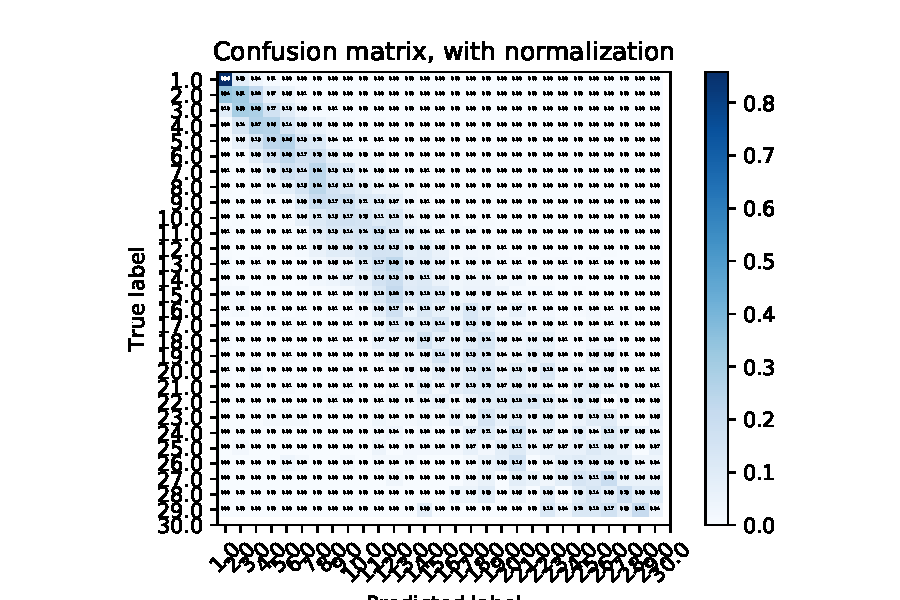
\includegraphics[scale=1]{../Figures/fig_iter1.pdf} \centering
  \caption{Confusion Matrix illustrating the first iteration of Stage2 LR. }
\end{figure} 



By looking at the confusion matrix the first thing we notice is data imbalance. Classes at the beginning have more supporting points, and therefore has less error than the others. However, class 2 has been identified as class 1 34\%. For example, the answer of \textit{At what age did Beyonce meet LaTavia Robertson?} is predicted as \textit{At age eight} while the correct answer is \textit{age eight}. Another example, the answer for \textit{How much was public expenditure on the island in 2001-2002?} is predicted to be \textit{Public expenditure} while the true answer is \textit{£10 million}. In this case, the phrase public expenditure appears in the question, which is a stronger candidate given the features designed. Similarly, class 12 is predicted as class eleven 16\%. For example, the answer to the question \textit{Who supervised the design and implementation of the iPod user interface?} is \textit{Steve Jobs}, but it is predicted as \textit{Of Steve Jobs}. Another example, answer to \textit{What roles were women recruited for in the 1950s?} is \textit{in medicine, communication}, but it is predicted as \textit{logistics, and administration}. Given the features we have designed it is very difficult for the classifier to recognize this settle difference between the classes. 


\subsection{Iteration 2}

In the first attempt we have sacrificed valuable data because the answer span was not within the constituents of the candidate sentence. This time, we use all 85K but we will face the same problem introduced in the previous section. The answer span can be a member of more than one constituent in the same sentence, and this will impose a very hard constraint on the performance because the inference can be close but not exact. Also because this problem requires more feature engineering efforts, we decided to leave it for future studies. Instead, we will set the target to the first constituent of which the span is a member. However, we will add three more features:

\begin{itemize}
\item \textbf{Distributional Distance}: We measure the distributional cosine similarity between the sum of all words in the contextual window and the question using Glove (Pennington, 2012). 

\item \textbf{Matching Word Frequencies}: Sum of the TF-IDF of the words that occur in both the question and the sentence containing the candidate answer.

\item \textbf{Lengths}: Number of words to the left and to the right of the span.
\end{itemize}

For classification we compare the performance of a logistic regression classifier with similar configuration as the first stage to 3-layer feed-forward neural network of 128, 64 and 32 nodes respectively. The logistic regression achieves 0.35 F1 while the neural network does 0.42 F1 using Adam optimizer and 100 epochs. Looking at the confusion matrix it is very clear that the new features (tf-idf and distributional cosine similarity) improve the performance. However, they could not recognize the settle difference among the phrase.  \\


\begin{figure}
  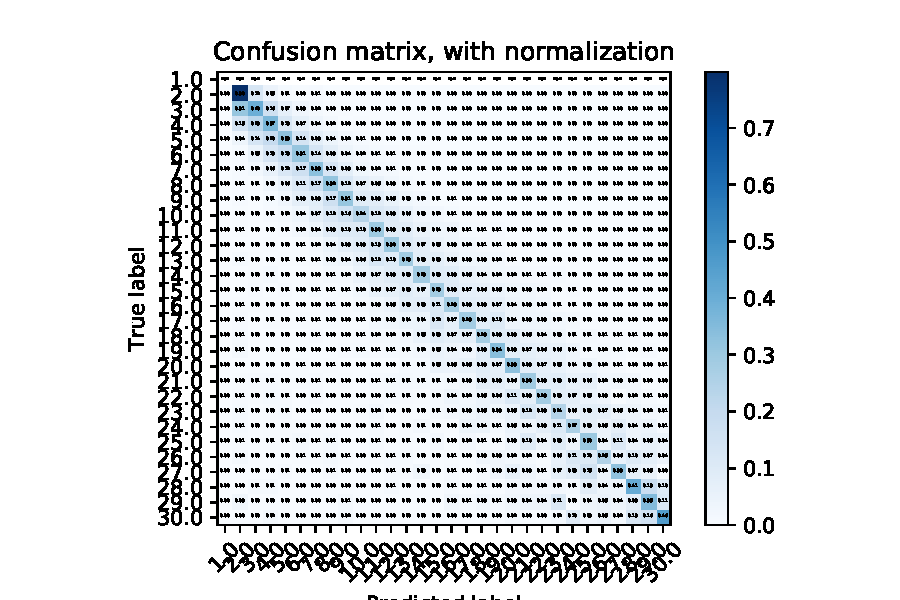
\includegraphics[scale=1]{../Figures/fig_1.pdf} 
  \caption{Confusion Matrix illustrating the Second iteration of Stage2 LR. }
\end{figure} 


\section{Conclusion}

We introduced a two-step classification method for automatic reading comprehension via SQUAD 2.0 dataset. Our stage1 classifier managed to find whether or not a question is answerable within a given passage and find the sentence containing the right answer with F1 score of 0.71. Our stage2 classifier manages to detect the exact span with F1 score of 0.35 even though the predicted answer is not distant from the exact answer. In order to improve the performance of our approach, future studies should investigate the usefulness of features generated from Named Entity Recognition, Semantic Role Labeling and Dependency Parsing processes, which are expected to be potential solutions to the problems we faced in this work. 
%% Chapter Template

\chapter{Two-stage Classification Method for Automatic Reading Comprehension } % Main chapter title

\label{Chapter3} % Change X to a consecutive number; for referencing this chapter elsewhere, use \ref{ChapterX}

\section{Introduction}

Teaching reading comprehension in an online learning environment is very challenging to the instructors as they need to provide the learners with reading material that is authentic, thematically diverse and appropriate to learners' reading level. The system we developed in the previous chapter help language instructors detect the grammatical difficulty of reading materials the find online, but it still does not help eliminate the efforts they need to expend on developing practice exercises and quizzes. In order for second and foreign language learners to master a difficult skill like reading comprehension, they need a lot of practice, which means more training exercises need to be prepared. So in this chapter we design and implement a system that automatically answers comprehension questions given a reading text. While such system still does not fully solve the problem raised, it can significantly aid in the automatic creation of reading comprehension practice activities in online learning environments. 

Automatic Reading Comprehension is the task of automatically answering comprehension questions based on information derived from short texts. Recently, it has received a special attention from NLP community because of the second release of Stanford Question Answering Dataset (SQuAD 2.0) \citep{rajpurkar2018know}. The dataset consists of 150K questions posed by crowd workers on a set of Wikipedia articles. The answers to these questions lie within the reading passages, though some questions are unanswerable from within the reading passage. What sets SQUAD 2.0 from other data sets is that 50k of its questions are unanswerable, and this requires the learning models not only to find answers, but also to abstain from answering when necessary. \\

The strategy we will use for this task is on two stages \ref{fig:arc-flowchart}. In the first stage, we break the reading passages into sentences, and train a multinomial logisitc regression classifier to find the sentence most likely contains the answer. We also train the classifier to give a null-answer if an answer does not exist. Next, we divide the best candidate sentence from stage one into its constituent phrases, and train another a multinomial logisitc regression classifier to find the constituent phrase that most likely to be the answer to the question. This dual stage method has advantages over other competing models when it comes to speed and consumption of computational resources. 

% The strategy will be used to tackle this task is mainly driven by pure linguistic intuition. Since SQUAD 2.0 task is a question answering task, the answer span lies within one of the given sentences in the paragraph, and then an answer is one of the constituents of the best candidate sentence. Thus, our goal is to, first, find the sentence containing the right answer, and we do by training a logistic regression classifier with some linguistic features. Then, we train another classifier to find the constituent best represent the right answer span within the sentence predicted in the first stage. In order to account for the unanswerability of some of the questions, we add a null-answer as a dedicated class in the first classifier along with the potential sentences. This way, if an answer is not found, the inference process stops without proceeding to the next stage, which saves time and computation. 



\section{Related Work}

There has been a large number of studies that tackle traditional Machine Comprehension tasks, where answers exist within the passage. The difficulty of SQUAD 2.0 task, though, lies in abstaining from answers when no answer span exists in the passage. Thus, in this section we review that models that address this constraint. It worth mentioning that all of the systems described in this section are complicated neural network architectures, and discussing its details is beyond the limitation of this report. 

\citep{DBLP:journals/corr/SeoKFH16} introduced bi-directional attention flow (BiDAF) that uses a recurrent neural network to encode contextual information in both question and passage along with an attention mechanism to align parts of the question to the sentence containing the answer and vise versa. The model offers context representation at multilevel of granularity: character-level, word-level, and contextual embedding. What sets this work from others is that it does not represent the context paragraph into a fixed-length vector. Instead, it dynamically computes vectors at each time step, combines it with the one from the previous layer and allow \textit{flow} through to the next layers. The model outputs confidence scores of start and end index of all potential answers. One problem with this model is that it is not designed to handle unanswerable questions. \citep{DBLP:journals/corr/LevySCZ17} extends the work by assigning a probability to null-answers to account for the questions whose answers do not exist in the corresponding paragraph. It achieves 59.2\% EM score and 62.1\% F1 score.\\

\citep{DBLP:journals/corr/abs-1808-05759} propose a read-then-verify system that can abstain from answering when a question has no answer given the passage. They introduce two auxiliary losses to help the neural reader network focus on answer extraction and no-answer detection respectively, and then utilize an answer verifier to validate the legitimacy of the predicted answer. One essential contribution is answer-verification. The model incorporates a multi-layer transformer decoder to recognize the textual entailment that supports the answer in and passage. This model achieves an ExactMatch EM score of 71.6\% and 74.23\% F1 on SQuAD 2.0. \\

\citep{DBLP:journals/corr/abs-1811-11934} proposes a new hierarchical attention network that mimics the human process of answering reading comprehension tests. It gradually focuses attention on the part of the passage containing the answer to the question. The modal comprises of three layers. a) \textbf{encoder layer}: builds representations to both the question and the passage using a concatenation of word-embedding representation \citep{pennington2014glove} and a pre-trained neural language modal \citep{Peters:2018} b) \textbf{Attention layer}: its function is to capture the relationship between the question and the passage at multiple levels using self-attention mechanisms. c) \textbf{Matching layer}: given refined representation for both question and passage, a bi-linear matching layer detects the best answer span for the question. This method achieves state-of-the-art results as of September 2018. Their single model achieves 79.2\% EM and 86.6\% F1 score, while their ensemble model achieves 82.4\% EM and 88.6\% F1 Score. \\

Current models that have shown significant improvement on Machine Comprehension tasks and other similar ones owe their success to a new neural architecture called transformer networks \citep{DBLP:journals/corr/VaswaniSPUJGKP17}. It has become the \emph{de facto} in recent sequential learning tasks, eschewing recurrence. This architecture creates global dependencies between input and output using only attention mechanisms. An even more successful model is Bidirectional Encoder Representations from Transformers BERT \citep{DBLP:journals/corr/abs-1810-04805}. It is a task-independent pretrained language model that uses a deep transformer network to create rich and context-specific vector representation. Using a method called Masked Language Model, the goal is to randomly mask tokens from the input and predict the vocabulary id of the masked word based only on its context. BERT has shown significant improvement on several tasks, one of which is SQUAD. 

While these models achieve astonishing results, they are very difficult to implement, and very resource-intensive. We argue that the simplifying linguistic assumptions we followed in our proposed strategy can greatly eliminate the need to such complexity of design, and yield good results. 

%The baseline for the task is a simple logistic regression with a set of features, and I would argue that adding more feature could achieve good results at a fracture of cost and complexity.

\section{Stage One: Selecting Best Candidate Sentence}

% The new version of SQuAD 2.0 task adds a new constraint to competing question-answering models. In addition to identifying the answer spans, a question-answering model should abstain from answering if the passage does not contain an answer. To this end, we implement a simple multinomial logistic regression classifier to address this task. 
At this level, the classification task is to predict the sentence, in the paragraph, containing the right answer, or declaring that the question is unanswerable. So we train a multiclass logistic regression classifier that takes a question and a reading passage as inputs and outputs the index of the passage sentence that is most likely contain the answer. The classifier is trained with L2 regularization and optimized using Newton-Raphson method. The best candidate sentence has the following three criteria. First, it shares more words with the question than other sentences. Second, it has high cosine similarity with the question than other sentences. Finally, it shares a syntactic similarity with the question. We are using these criteria as features for the classifier. 

% Next, we apply a constituency parser over the sentence predicted from the first stage to get its constituents among which lies the correct answer span (see Figure 1).  

\begin{figure}
  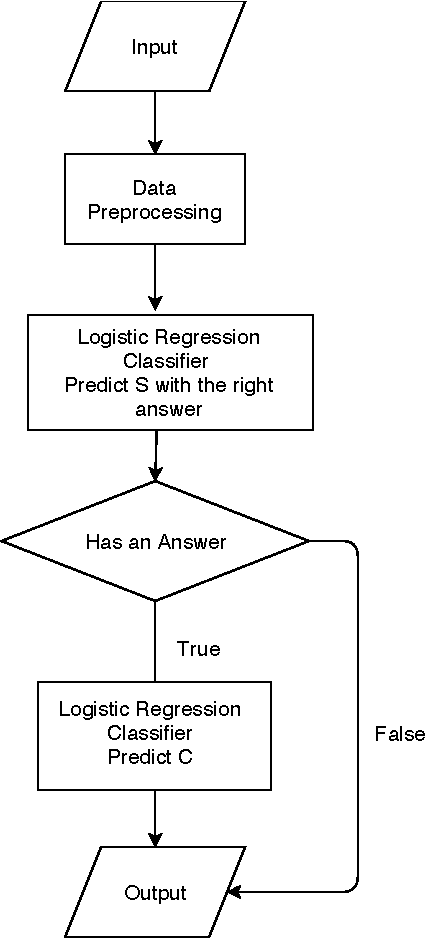
\includegraphics[scale=1]{../Figures/Flowchart.pdf}\centering
  \caption{Flowchart illustrating the two-stage classification approach}
  \label{arc-flowchart}
\end{figure}


\subsection{Feature Extraction} 
% In order for the classifier to find the sentence containing the answer, it must determine the sentence that is most similar to the question, and by similar we mean that a good candidate sentence  1) shares more words with the question. 2) has high cosine similarity with the question. 3) shares a syntactic similarity with the question. Thus, three main features have been selected to this end:
\begin{itemize}
\item \textbf{Cosine Similarity}: for every sentence in the paragraph as well as the question a word vector representation is created via InferSent (Conneau et al, 2017), which is a pre-trained sentence embeddings method that provides semantic representations for English sentences. InferSent is an encoder based on a bi-directional LSTM architecture with max pooling, trained on the Stanford Natural Language Inference (SNLI) dataset. Cosine distance score is calculated for each sentence-question pair. 
\item \textbf{Word Overlap}: calculates the Jaccard score between each sentence-question pair. Jaccard index is a method of computing the explicit similarity between two sets as follows: 
$$
J(Q,S) = \frac{|Q \cap S|}{|Q \cup S|}
$$
where Q and S are sets of words in question and sentence respectively.

\item \textbf{POS Overlap}: computes the Jaccard score over the part-of-speech-tag representation of sentences. In other words, instead of the word tokens, it checks similarity over POS tokens. We use the default POS-tagger in the SpaCy library of Python programming language to obtain the POS representation for the sentences and questions alike.
\end{itemize}
Using the three features above every question-sentence pair will have three scores and an additional binary feature indicating whether or not the question is answerable. 

\subsection{Training and Result} 
 We get the results shown in \ref{table:mlr-stage1}. Numbers in class column represents the index of the sentence in the paragraph containing the answer, and -1 indicates that the question has no answer in the paragraph. We also limit the number of sentences to 10. The results show that with simple features we get an F1 score of 0.71.

\begin{figure}
  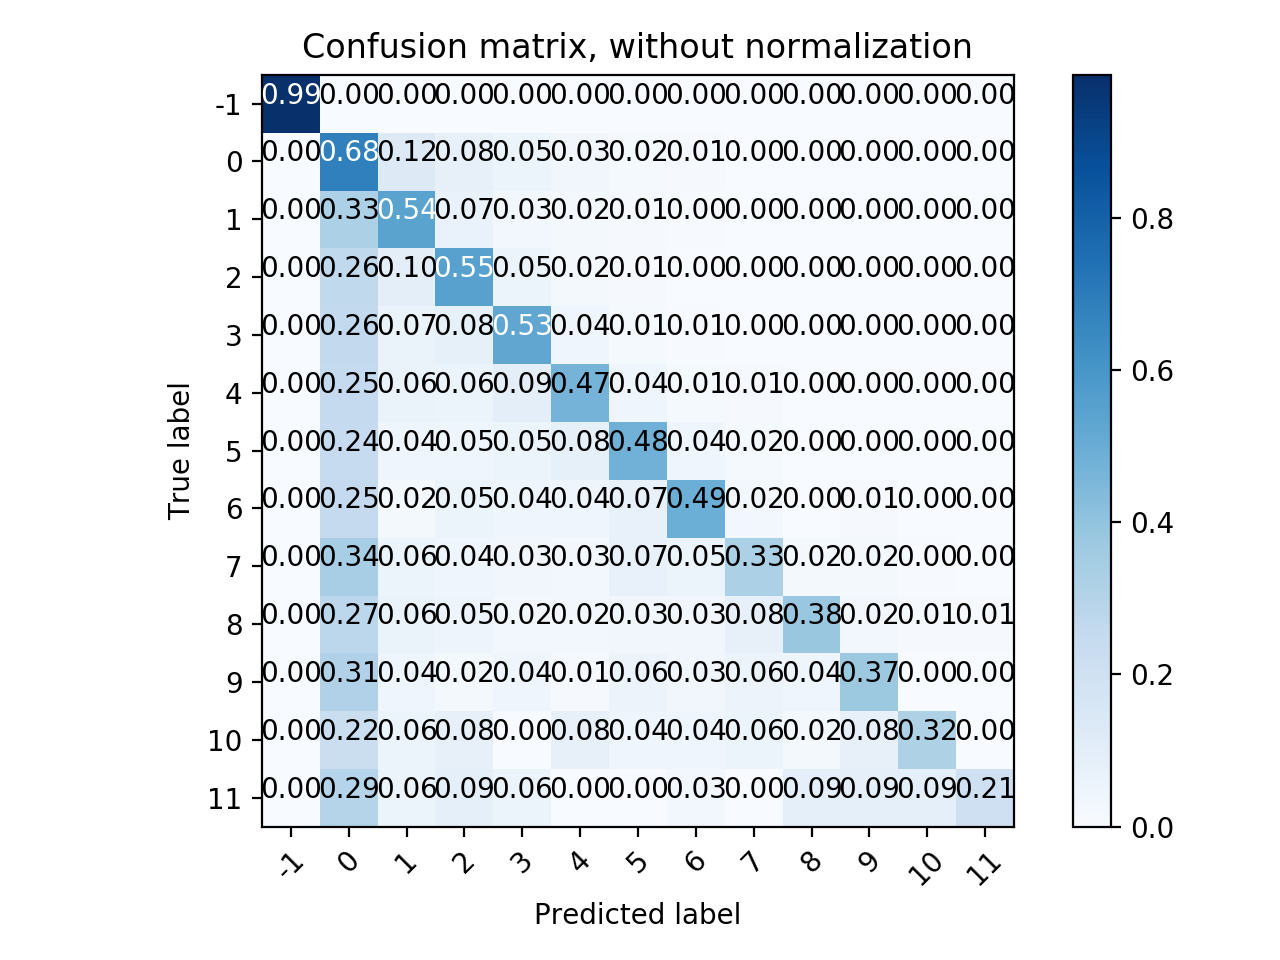
\includegraphics[scale=1]{Figure_1.png}\centering
  \caption{Confusion matrix shows which classes were predicted correctly}
\end{figure}

\begin{table}
\centering
\caption{This table shows the results of running a multinomial regularized logistic regression. The class column represents the index of sentences within the paragraph, and -1 represents the unanswerable question case. Unpredicted classes are removed.}
\label{mlr-stage1}
\begin{tabular}{|l|l|l|l|} 
\hline
 \textbf{class}  & \textbf{precision}  & \textbf{recall}  & \textbf{F1-score}   \\ 
\hline
-1               & 1                   & 0.99             & 0.99                \\ 
\hline
0                & 0.47                & 0.68             & 0.56                \\ 
\hline
1                & 0.63                & 0.54             & 0.58                \\ 
\hline
2                & 0.62                & 0.55             & 0.58                \\ 
\hline
3                & 0.62                & 0.53             & 0.57                \\ 
\hline
4                & 0.58                & 0.47             & 0.52                \\ 
\hline
5                & 0.57                & 0.48             & 0.52                \\ 
\hline
6                & 0.57                & 0.49             & 0.53                \\ 
\cline{1-3}
7                & 0.46                & 0.33             & 0.38                \\ 
\hline
8                & 0.56                & 0.38             & 0.45                \\ 
\hline
9                & 0.46                & 0.37             & 0.41                \\ 
\hline
10               & 0.48                & 0.32             & 0.39                \\ 
\hline
11               & 0.35                & 0.21             & 0.26                \\ 
\hline
avg / total      & 0.72                & 0.71             & 0.71                \\
\hline
\end{tabular}
\end{table}

\newpage

\section{Stage Two: Predicting the Answer Span}

Stage Two: Selecting the Answer Span
To select the most plausible answer span from the candidate sentence, we design a number of features, some of which are based on constituent analysis. A constituency parser is used to analyze a sentence into its constituent phrases. For example, the sentence "the quick brown fox jumps over the lazy dog" has the following syntactic (constituency) tree:


The intuition is an answer span is one of constituents of the best candidate sentence. So we are using a constituency parser (Kitaev and Klein, 2018), we obtain all constituents in a candidate sentence. These constituents will be the classes from which we pick the right span. More generally, we design the following features for this stage:

\begin{itemize}
\item \textbf{Contextual Overlap}: Constituents sharing context with the original question are potential candidates to be the correct answers. So we measure the cosine similarity between each constituent and the question:

$${ similarity } = \frac { \sum _ { i = 1 } ^ { n } C _ { |w| } Q _ { i } } { \sqrt { \sum _ { i = 1 } ^ { n } C _ { |w| } ^ { 2 } } \sqrt { \sum _ { i = 1 } ^ { n } Q _ { i } ^ { 2 } } }$$ 

where w is the number of slide window around the candidate constituent. For our purposes features of size 2 and 3 are used.


\item \textbf{Constituent Label}: Constituency parse tree label of the span combined with wh-word. For example, for a question "who designed the iPhone prototype?" and its answer "Steve Jobs designed the first prototype for the iPhone.", a constituent label feature is {who-NP, who-V, who-VP, who-PP, etc}. 
\item \textbf{Distributional Distance}: We measure the distributional cosine similarity between the sum of all words in the contextual window and the question using Glove (Pennington, 2012).
\item \emph{Matching Word Frequencies}: Sum of the TF-IDF of the words that occur in both the question and the sentence containing the candidate answer.
\item \emph{Lengths}: Number of words to the left and the right of the span.
\end{itemize}

\section{Experiment and Error Analysis}
In this stage, we have done three different attempts. 
In the first attempt, we used only two features "contextual overlap" and "constituent label". We also limited the number of classes (constituents) to 30. Using the same training settings and configurations from stage one, the logistic regression achieves a 0.25 F1 score. The confusion matrix shows a clear case of data imbalance. Classes at the beginning have more supporting points, and therefore have less errors than others. However, our analysis to the errors indicate the wrong answers are partially correct most of the times. class 2 has been identified as class 1 34\%. For example, the answer of \emph{At what age did Beyonce meet LaTavia Robertson? }is predicted as \emph{At age eight} when the correct answer is \emph{age eight}. Similarly, class 12 is predicted as class eleven 16\%. The answer to the question \emph{Who supervised the design and implementation of the iPod user interface?} is \emph{Steve Jobs}, but it is predicted as \emph{Of Steve Jobs}. Clearly, the predicted answers are not very far from the true ones. A harsher assumption such as keeping only Noun Phrase constituents could have resolved some of these issues, but we will leave this for future studies. 

Other types of errors are due to literal word matching between the questions and phrases. For example, the answer for \emph{How much was public expenditure on the island in 2001-2002?} is predicted to be \emph{Public expenditure} when the true answer is \emph{£10 million}. In this case, the phrase \emph{public expenditure} appears in the question, which makes it a stronger candidate given the features designed. Another example, answer to \textit{What roles were women recruited for in the 1950s?} is \emph{in medicine, communication}, but it is predicted as \emph{logistics, and administration}. Given the features we have designed, it is very difficult for the classifier to recognize this settle difference between the classes. 
In the second attempt, we have added the 3 remaining features: Distributional Distance, Matching Word Frequencies, and length, while keeping the same parameters of the first attempt. We get a 0.35 F1 score. Looking at the confusion matrix, it is apparent that the new features do significantly improve the performance.

In our last experiment, we replaced logistic regression classifier in second attempt with a 3-layer feed-forward neural network of 128, 64 and 32 nodes respectively, optimized by Adam optimizer on a 100 epochs . The neural network achieves F1 score of 0.42. Using a neural network does indeed increase the performance, but its use is not very practical given its configuration. Each node in this neural network is equivalent to one logistic regression classifier, so using a feed-forward neural network with a total nodes of 224 is equal in computational power to 224 logistic regression. 

\section{Future Studies and Recommendation}
Looking at errors produced during the three attempts, we can improve the performance by injecting more linguistic information from Named Entity Recognizers, Semantic Role Labelers and Dependency Parsers. A Named Entity Recognizer can help answer questions about locations, persons or entities (Where, Who and Which questions). Information derived from a dependency parser and a semantic role labeler can, for example, help resolve cases when the answers are the subjects or the objects of the sentences. Another thing to investigate is to eliminate PP and VP constituent phrases, and only keep NP phrases. This idea comes from the assumption that the majority of answers to Wh-questions in SQUAD 2.0 dataset can be Noun Phrases.This assumption can help reduce the number of classes to be predicted, and there will be no need to limit the number of outputs to certain number as we did.

\section{Conclusion}
We introduced a two-step classification method for automatic reading comprehension via SQUAD 2.0 dataset. Our stage 1 classifier managed to find whether or not a question is answerable within a given passage and find the sentence containing the right answer with F1 score of 0.71. Our stage 2 classifier manages to detect the exact span with F1 score of 0.35 even though the predicted answer is not distant from the exact answer. In order to improve the performance of our approach, future studies should investigate the usefulness of features generated from Named Entity Recognition, Semantic Role Labeling and Dependency Parsing processes, which are expected to be potential solutions to the problems we faced in this work

%\subsection{First Attempt}
%To select the most plausible answer span from the candidate sentence, we design a number of features:
%\begin{itemize}
%\item \textbf{Constituents}: Using a constituency parser \citep{kitaev2018constituency}, we obtain all constituents in a candidate sentence. These constituents will be the classes from which we pick the right span.
%\item \textbf{Contextual Overlap}: Constituents sharing context with the original question are potential candidates to be the correct answers. So we measure the cosine similarity between each constituent and the question:
%$${ similarity } = \frac { \sum _ { i = 1 } ^ { n } C _ { |w| } Q _ { i } } { \sqrt { \sum _ { i = 1 } ^ { n } C _ { |w| } ^ { 2 } } \sqrt { \sum _ { i = 1 } ^ { n } Q _ { i } ^ { 2 } } }$$ 
%where $w$ is the number of slide window around the candidate constituent. For our purposes features of size 2 and 3 are used. 
%
%\item \textbf{Constituent Label}: Constituency parse tree label of the span combined with wh-word.
%\end{itemize}
%Out of 85K training example, the answer spans of nearly half of them are not within the constituents. However, answers can be part of the constituents.  For example, an answer span might be \textit{L'official} and the nearest constituent is \textit{L'official Magazine}. So for our first attempt, we remove all data points whose answers are not explicitly found within the constituents. This results in around 45K data point. Next, we train a logistic regression classifier with L2 regularization and 100 epochs, optimized by newton method 'newton-cg' on a MacBook Pro laptop with core i5 processor and 8 GB of RAM. Python modules used are Scikit-learn and SpaCy. The latter is used to drive the attentive-neural constituency parser (Kitaev, 2018). The result is 0.25 F1 score.
%
%
%
%
%\subsection{Error Analysis of First Attempt}
%%\subsection{Format of Electronic Manuscript}
%%\label{sect:pdf}
%
%\begin{figure}
%  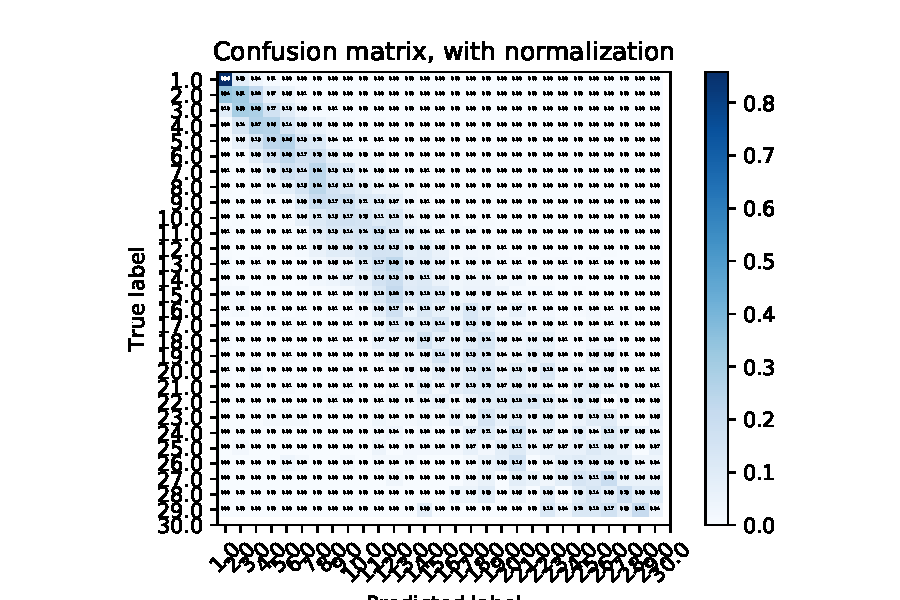
\includegraphics[scale=1]{../Figures/fig_iter1.pdf} \centering
%  \caption{Confusion Matrix illustrating the first iteration of Stage2 LR. }
%\end{figure} 
%
%
%
%Looking at the confusion matrix, we notice that there is a data imbalance. Classes at the beginning have more supporting points, and therefore have less error than the others. However, class 2 has been identified as class 1 34\%. For example, the answer of \textit{At what age did Beyonce meet LaTavia Robertson?} is predicted as \textit{At age eight} while the correct answer is \textit{age eight}. Another example, the answer for \textit{How much was public expenditure on the island in 2001-2002?} is predicted to be \textit{Public expenditure} while the true answer is \textit{£10 million}. In this case, the phrase public expenditure appears in the question, which is a stronger candidate given the features designed.
%Similarly, class 12 is predicted as class eleven 16\%. For example, the answer to the question \textit{Who supervised the design and implementation of the iPod user interface?} is \textit{Steve Jobs}, but it is predicted as \textit{Of Steve Jobs}. Another example, answer to \textit{What roles were women recruited for in the 1950s?} is \textit{in medicine, communication}, but it is predicted as \textit{logistics, and administration}. Given the features, we have designed it is very difficult for the classifier to recognize this settle difference between the classes. 
%
%
%\subsection{Second Attempt}
%
%In the first attempt, we have sacrificed valuable data because the answer span was not within the constituents of the candidate sentence. This time, we use all 85K, but we will face the same problem introduced in the previous section. The answer span can be a member of more than one constituent in the same sentence, and this will impose a very hard constraint on the performance because the inference can be close but not exact. Also because this problem requires more feature engineering efforts, we decided to leave it for future studies. Instead, we will set the target to the first constituent of which the span is a member. However, we will add three more features:
%
%\begin{itemize}
%\item \textbf{Distributional Distance}: We measure the distributional cosine similarity between the sum of all words in the contextual window and the question using Glove (Pennington, 2012). 
%
%\item \textbf{Matching Word Frequencies}: Sum of the TF-IDF of the words that occur in both the question and the sentence containing the candidate answer.
%
%\item \textbf{Lengths}: Number of words to the left and the right of the span.
%\end{itemize}
%
%For classification, we compare the performance of a logistic regression classifier with a similar configuration as the first stage to 3-layer feed-forward neural network of 128, 64 and 32 nodes respectively. The logistic regression achieves 0.35 F1 while the neural network does 0.42 F1 using Adam optimizer and 100 epochs. Looking at the confusion matrix, it is apparent that the new features (tf-idf and distributional cosine similarity) improve the performance. However, they could not recognize the settle difference among the phrase.  \\
%
%
%\begin{figure}
%  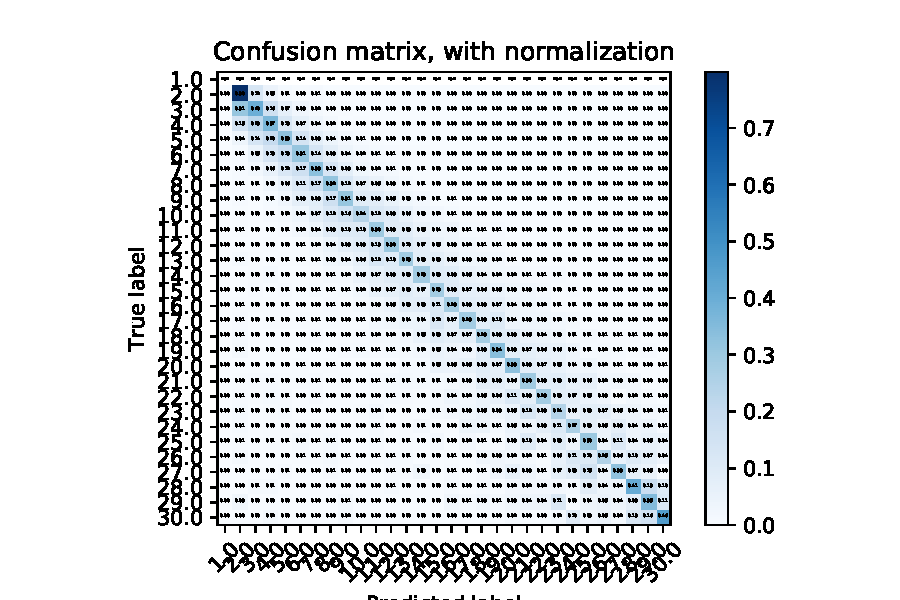
\includegraphics[scale=1]{../Figures/fig_1.pdf} 
%  \caption{Confusion Matrix illustrating the Second iteration of Stage2 LR. }
%\end{figure} 
%
%
%\section{Conclusion}
%
%We introduced a two-step classification method for automatic reading comprehension via SQUAD 2.0 dataset. Our stage1 classifier managed to find whether or not a question is answerable within a given passage and find the sentence containing the right answer with F1 score of 0.71. Our stage2 classifier manages to detect the exact span with F1 score of 0.35 even though the predicted answer is not distant from the exact answer. In order to improve the performance of our approach, future studies should investigate the usefulness of features generated from Named Entity Recognition, Semantic Role Labeling and Dependency Parsing processes, which are expected to be potential solutions to the problems we faced in this work.  
%% Chapter Template

\chapter{Conclusion} % Main chapter title

\label{Chapter5} % Change X to a consecutive number; for referencing this chapter elsewhere, use \ref{ChapterX}

Applications of Machine Learning in education are ubiquitous, from learning analytics to machine translation to summarization. One field of education that can be greatly benefited from the applications of natural language processing is distance education. Teaching foreign languages by means of distance learning requires tremendous efforts from instructors and course developer to prepare online materials, learning activities and resources.   This report examines the applicability of supervised classification technique called logistic regression in two educational scenarios: detection of grammatical difficulty and automatic reading comprehension. The simplicity and practicality of the proposed solutions to each of these problems make them uniquely useful in onsite and online teaching environments. 

As we pointed out in chapter 2, representing a written text is a crucial step in the machine learning pipeline, and to do so, we have explored some of the most common methods such as bag-of-word, TF-IDF, and word embeddings.  We have also noticed the advantages and disadvantages of each method in addition to techniques of dimensionality reduction such as clustering, latent semantic allocation, and stemming and lemmatization. Moreover, we have explained the workflow of classification as a supervised machine learning, starting from feature extraction through classification to evaluation of performance. 

In chapter 3, we examine the use of multinomial logistic regression classifier to classify a written text according to how difficult a foreign language learner of English sees it using educational standards of Common European Framework Reference (CEFR). We also showed how logistic regression classifier could fit within a semi-supervised framework such as bootstrapping to work on low resources data. 

In Chapter 4, we have investigated another use for logistic regression classification in method on a novel educational task, automatic reading comprehension. We have demonstrated that using logistic regression on two stages can compete with relatively advanced and complex neural network architecture commonly used for this purpose. The main catalyst for this success comes from using a set of linguistically rich features such as constituency parser and sentential embeddings. The performance of the model, the analysis of error made as well as the simplicity and efficiency of the model make it feasible to be applied in onsite or virtual learning environments.


\section{Summary of Contributions}

There are three main contributions to this work. First, we are, to the best of our knowledge, the first to propose an automated solution to classify a written English text by following pedagogic standards (CEFR). Second, we have \emph{cautiously} applied a bootstrapping technique to supplement the training data from unlabeled corpora, and that led to 10\% F1 increase in performance. Finally, we created a novel two-stage system based on multinomial logistic regression that not only answers comprehension questions given reading passages but it also able to abstain from answering if a question is unanswerable within the reading passage. 

%-----------------------------------
%    SUBSECTION 1
%-----------------------------------
\section{Recommendations and Future Work}

We have seen that each of the tasks we tackled in this report can help solve a particular educational scenario a foreign language instructor may encounter in a face-to-face or online learning settings. However, there still exist a few challenges that need the attention of NLP researchers. The solution proposed in chapter 4 find answers to comprehension questions, but it still requires the questions as input. This means, teachers and material developers still have to create the questions. Thus, future studies are to investigate the process of automatically creating different types of comprehension questions given reading passages. Such a system, complemented by the system we proposed, can make an automatic tool of learning activity creation that is ready to deploy in Learning Management Systems (LMS) or Courseware Platforms. As for improving the performance of the current automatic reading comprehension system, we recommend incorporating more linguistic features such as information derived from Named Entity Recognition, Dependency Parsing and Semantic Role Labeling. 

Due to the shortage of training examples on each of six classes in the grammatical detection task, we merged every two classes into one super-class to be the output. However, to provide more specificity to error detection, we recommend applying more iterations of cautious bootstrapping to obtain more training examples on each of the six classes (A1, A2, B1, B2, C1, C3). More training examples can also reduce the state of data imbalance we had in this task, and therefore could eliminate the need for adjusting the class weights. The features we used are based on bag-of-words and TFIDF, and we recommend using word embeddings or the sentence embeddings technique we have used for automatic reading comprehension task in chapter 4. Another recommendation is to use easy-to-interpret classification algorithms like decision trees. This brings the advantage of providing "if-then" classification rules that humans can read and understand. Furthermore, as the task involves grammatical structures, we recommend designing features using constituency and dependency parsers. Finally, we encourage future studies to investigate how close will be the rules generated from the last two recommendations to the ones CEFR experts devised (can-do statements). 


 

%----------------------------------------------------------------------------------------
%	THESIS CONTENT - APPENDICES
%----------------------------------------------------------------------------------------

\appendix % Cue to tell LaTeX that the following "chapters" are Appendices

% Include the appendices of the thesis as separate files from the Appendices folder
% Uncomment the lines as you write the Appendices

\chapter{Auxiliary Functions for Codes in Ch3\&4} % Main appendix title

\label{AppendixA} % For referencing this appendix elsewhere, use \ref{AppendixA}

\lstset{language=Python}
\lstset{frame=lines}
\lstset{caption={Helper Functions for Tokenization, Projection and Plotting}}
\lstset{label={lst:code_direct}}
\lstset{basicstyle=\footnotesize}

\lstinputlisting[language=Python]{Appendices/aux_functions.py}
%\chapter{Complete Code for Grammatical Detection System} % Main appendix title

\label{AppendixB} % For referencing this appendix elsewhere, use \ref{AppendixA}

\lstset{language=Python}
\lstset{frame=lines}
\lstset{caption={Helper Functions for Tokenization, Projection and Plotting}}
\lstset{label={lst:code_direct}}
\lstset{basicstyle=\footnotesize}

\lstinputlisting[language=Python]{Appendices/ch3_grammar_detection.py}
%\chapter{Complete Code for Automatic Reading Comprehension} % Main appendix title

\label{AppendixC} % For referencing this appendix elsewhere, use \ref{AppendixA}

\lstset{language=Python}
\lstset{frame=lines}
% \lstset{caption={Helper Functions for Tokenization, Projection and Plotting}}
\lstset{label={lst:code_direct}}
\lstset{basicstyle=\footnotesize}

\lstinputlisting[language=Python]{Appendices/ch4_preprocess.py}
\lstinputlisting[language=Python]{Appendices/ch4_stage1.py}
\lstinputlisting[language=Python]{Appendices/ch4_stage2.py}

%----------------------------------------------------------------------------------------
%	BIBLIOGRAPHY
%----------------------------------------------------------------------------------------

\printbibliography[heading=bibintoc]

%----------------------------------------------------------------------------------------

\end{document}  
